% !TEX program = lualatex
\documentclass[a4paper,11pt]{report}
\usepackage[a4paper,left=23mm,right=23mm,top=24mm,bottom=24mm]{geometry}
\usepackage[english,main=english]{babel}
\usepackage{fontspec}
\usepackage[autostyle]{csquotes}
\usepackage{microtype}
\usepackage{amsmath}
\usepackage{graphicx}
\usepackage{tabularx}
\usepackage{booktabs}
\usepackage{array}
\usepackage{siunitx}
\usepackage{xcolor}
\usepackage{float}
\usepackage[parfill]{parskip}
\usepackage[hypertexnames=false,colorlinks=true,linkcolor=blue,urlcolor=blue]{hyperref}
\sisetup{group-digits=integer}
\newcommand{\opamp}{OPAMP}
\newcommand{\VDD}{V_{\mathrm{DD}}}
\newcommand{\VCM}{V_{\mathrm{CM}}}
\newcommand{\Ron}{R_{\mathrm{on}}}
\newcommand{\Roff}{R_{\mathrm{off}}}
\newcolumntype{Y}{>{\raggedright\arraybackslash}X}
\newcolumntype{C}{>{\centering\arraybackslash}X}
\hypersetup{pdftitle={Programmable-Gain Analog Front End},pdfauthor={Qi Wu and one teammate},pdfsubject={AICD Lab portfolio edition}}
\begin{document}
\begin{titlepage}
\raggedright
\vspace*{24mm}
{\large Advanced Integrated Circuit Design Lab\par}
\vspace{12mm}
{\Huge\bfseries Programmable-Gain\\[3mm]Analog Front End\par}
\vspace{8mm}
{\Large OPAMP, PGA, and Active Low-Pass Filter\par}
\vspace{16mm}
{\large Qi Wu and one teammate\par}
TU Darmstadt\par
Summer semester 2026\par
\vfill
\textbf{Portfolio edition}\par
This report documents the group's schematic design and archived simulation results. Teammate layout images and physical-verification screenshots are omitted from this portfolio edition. The contribution statement identifies each student's work.\par
Nominal, corner, and Monte Carlo results are schematic-level results. Complete extracted-view and PEX performance results are not available.\par
\end{titlepage}
\chapter*{Abstract}
\addcontentsline{toc}{chapter}{Abstract}

This report presents a programmable-gain analog front end for a \SI{1.8}{V} supply. It combines a two-stage Miller-compensated OPAMP, an eight-step inverting PGA, a CMOS transmission-gate multiplexer, a Verilog-A 3-to-8 one-hot controller, and a first-order active low-pass filter (LPF). At \(\VCM=\SI{0.9}{V}\) with a \SI{2}{pF} load, the OPAMP achieves \SI{79.93}{dB} DC gain, \SI{51.31}{MHz} gain-bandwidth product, \SI{61.97}{\degree} phase margin, and \SI{0.3113}{mW} power dissipation. Within the specified \SIrange{0.5}{1.3}{V} ICMR, the maximum unity-follower error is \SI{0.8503}{mV}, below the \SI{50}{mV} limit. All 12 expressions in the 64-corner export pass at every corner. In the 1000-point Monte Carlo analysis, the offset yield is 972/1000; the other exported metrics pass 1000/1000.

The simulated OPAMP output swing is approximately \SIrange{0.430}{1.401}{V} and does not cover the full specified \SIrange{0.3}{1.5}{V} range. However, all eight PGA settings from 0 to \SI{21}{dB} remain within the \(\pm\SI{1.5}{dB}\) limits at nominal conditions, across 64 corners, and for 100 Monte Carlo samples per code under the applied stimuli. The worst measured switch resistances are \(\Ron=\SI{232.1}{\ohm}\) and \(\Roff=\SI{38.81}{\giga\ohm}\). The LPF bandwidth is \SI{100.1}{kHz} nominally, \SIrange{72.88}{121.8}{kHz} across corners, and \SIrange{82.8}{119.5}{kHz} in Monte Carlo analysis. This portfolio is limited to schematic work. Teammate layout and physical-verification images are omitted, and no post-layout performance is claimed.

\tableofcontents
\chapter{Introduction}

\section{Design objective}

We designed a programmable-gain analog front end consisting of an OPAMP, an eight-step PGA, and an active LPF. The PGA adjusts the signal amplitude for the following ADC, while the LPF limits out-of-band content. We set \(\VDD=\SI{1.8}{V}\) and \(\VCM=\SI{0.9}{V}\), with a load of at least \SI{2}{pF}.

The PGA performance depends directly on the OPAMP output range, stability, load capability, and offset. The layout must preserve the simulated resistor ratios, switch dimensions, controller behavior, and LPF values. We therefore report the schematic design first, together with its nominal, PVT-corner, and Monte Carlo verification.

\section{Specifications and verification}

Numerical values come from the Cadence ADE exports. Screenshots document circuit configurations and waveform trends; where labels are small, the exported scalar values are used instead of numbers read from the image. Table~\ref{tab:requirements} summarizes the OPAMP requirements and measurement methods given in the course documents.

\begin{table}[htbp]
\centering
\caption{OPAMP design requirements and verification methods.}
\label{tab:requirements}
\small
\renewcommand{\arraystretch}{0.92}
\begin{tabularx}{\textwidth}{@{}Y C Y@{}}
\toprule
Metric & Requirement & Verification method \\
\midrule
DC gain & $>\SI{50}{dB}$ & AC/STB analysis \\
Gain-bandwidth product & $\geq\SI{20}{MHz}$ & AC/STB analysis \\
Phase margin & $\geq\SI{55}{\degree}$ & STB analysis \\
CMRR & $>\SI{60}{dB}$ & common-mode small-signal analysis \\
Positive/negative slew rate & each $\geq\SI{15}{V/\micro s}$ & large-signal transient \\
High/low settling time & each $\leq\SI{500}{ns}$ at 5\% & large-signal transient \\
Input common-mode range & \SIrange{0.5}{1.3}{V} & unity-follower error $<\SI{50}{mV}$ over the specified interval \\
Output swing & \SIrange{0.3}{1.5}{V} & output sweep/transient \\
Input offset & $\leq\SI{5}{mV}$ absolute & DC and Monte Carlo \\
Input noise & $\leq\SI{55}{nV/\sqrt{Hz}}$ at \SI{20}{kHz} & noise analysis \\
Power & $\leq\SI{0.6}{mW}$ & supply-current measurement \\
Area & report value & extracted layout \\
\bottomrule
\end{tabularx}
\renewcommand{\arraystretch}{1}
\end{table}

The PGA targets 0 to \SI{21}{dB} in \SI{3}{dB} steps with a tolerance of $\pm\SI{1.5}{dB}$, while the LPF targets \SI{100}{kHz} within the allowed \SIrange{50}{150}{kHz} range. This portfolio excludes teammate layout and physical-verification images. Chapter~4 states the scope and remaining verification work.

\chapter{OPAMP Design and Verification}

\section{Architecture and schematic}

The core is a two-stage Miller-compensated OPAMP. M1/M2 form the NMOS differential pair, M3/M4 the PMOS current-mirror load, and M5 the tail-current source. The second stage uses PMOS M6 as a common-source device and NMOS M7 as its current-source load. M8 and the series bias resistors $R_0$/$R_2$ generate the bias voltage for M5 and M7. A series $R_Z$--$C_C$ branch from the first-stage node to the output provides frequency compensation.

\begin{figure}[htbp]
\centering
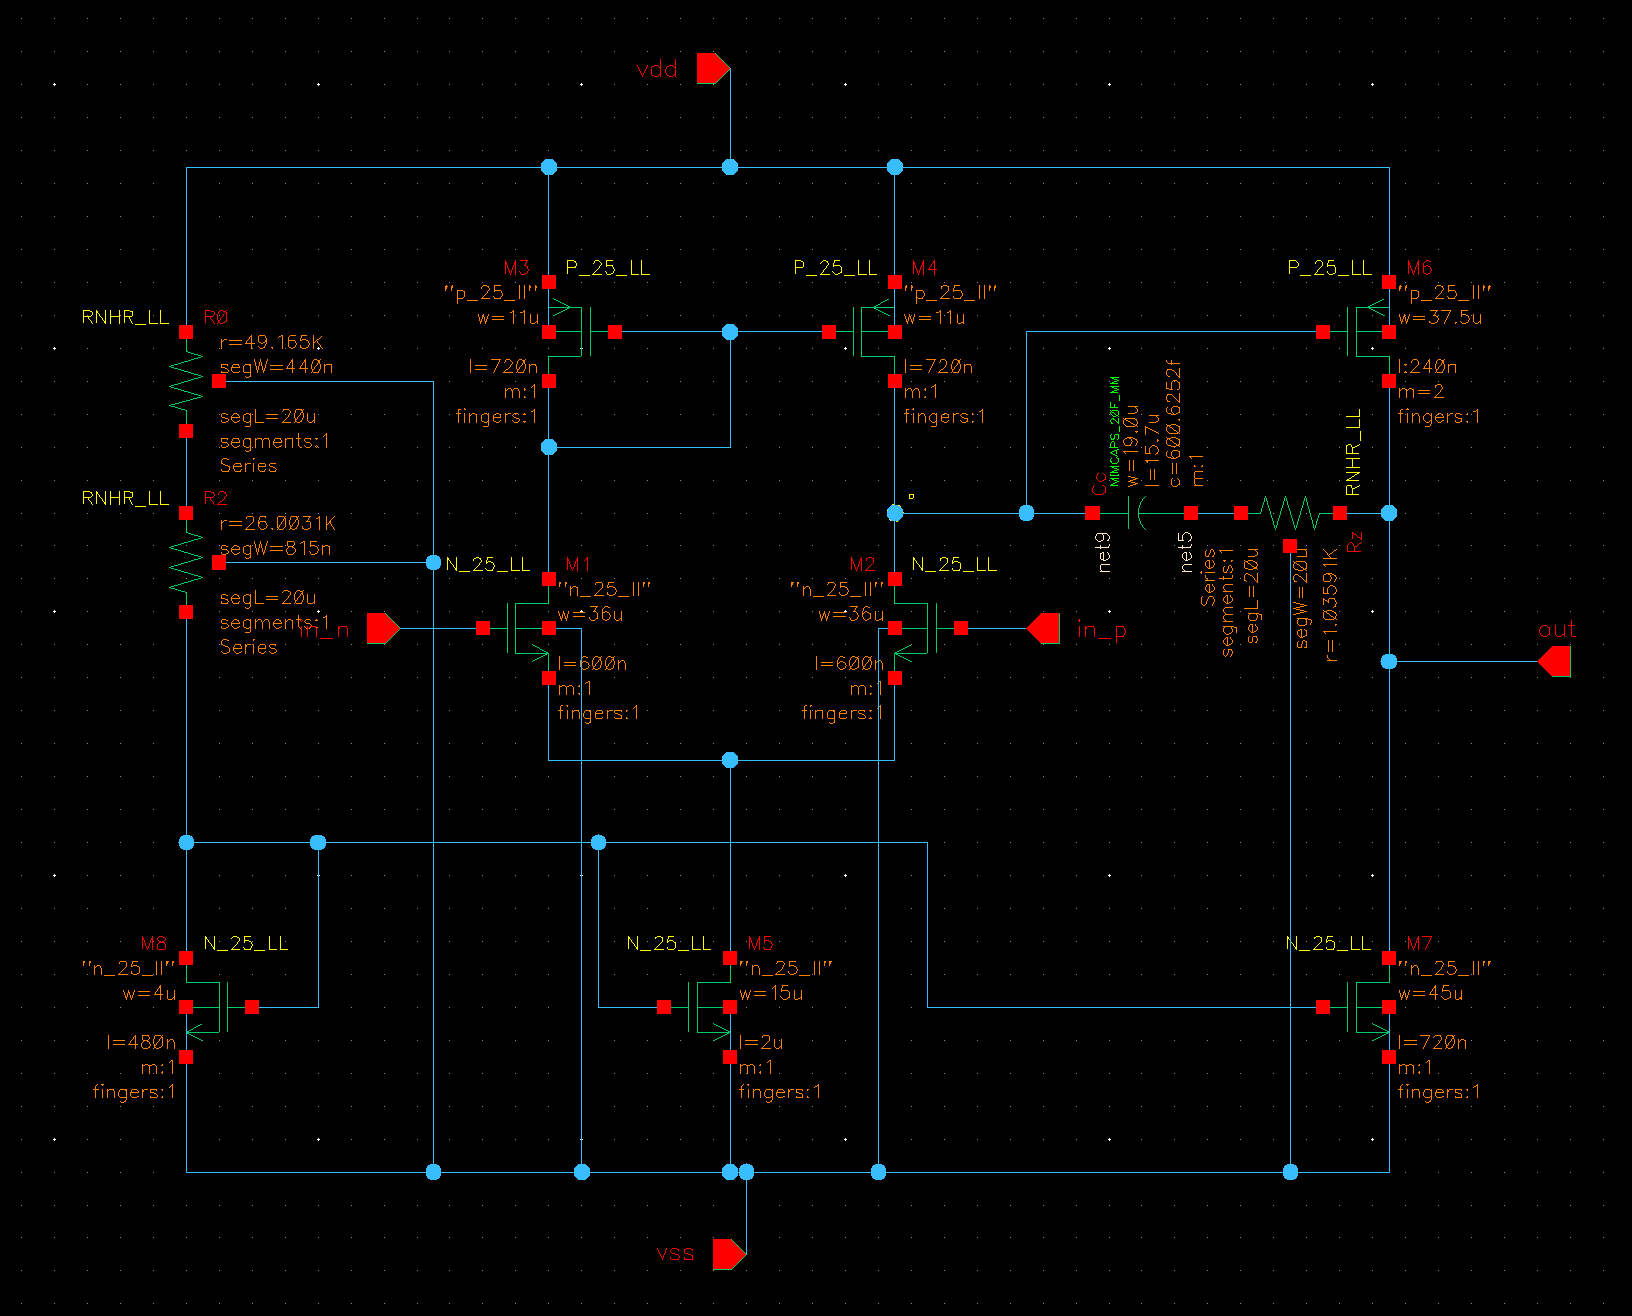
\includegraphics[width=\textwidth]{figures/opamp/schematic_final.png}
\caption{OPAMP schematic corresponding to the archived simulation baseline.}
\label{fig:final-schematic}
\end{figure}

The schematic interface is \texttt{in\_n}, \texttt{in\_p}, \texttt{out}, \texttt{vdd}, and \texttt{vss}. Figure~\ref{fig:final-schematic} shows the simulated schematic baseline. The verified results in this chapter use the same topology and interface together with the frozen schematic baseline values stated below, a \SI{1.8}{V} supply, a \SI{0.9}{V} input common-mode voltage, and a \SI{2}{pF} load.

\section{Hand calculation, sizing, and operating point}
\label{sec:final-design}

For the initial sizing, we fixed the channel length $L$, selected the target $g_m/I_D$, read the corresponding current density $I_D/W$, and calculated $W=I_D/(I_D/W)$. The hand calculation covers M1--M7; the M8 entry remains incomplete. Table~\ref{tab:sizing} compares these width targets with the first implementation and the final dimensions.

\begin{table}[htbp]
\centering
\caption{OPAMP sizing progression for the simulated schematic baseline (course Table~1). Dimensions are in \si{\micro m}; $L_{\min}=\SI{0.24}{\micro m}$.}
\label{tab:sizing}
\small
\resizebox{\textwidth}{!}{%
\begin{tabular}{@{}lrrrllr@{}}
\toprule
Device & Hand $g_m/I_D$ (V$^{-1}$) & Hand $I_D/W$ (\si{\micro A/\micro m}) & Hand $W$ target & First $W/L$ & Final effective $W/L$ & $L/L_{\min}$ \\
\midrule
M1/M2 & 17.049 & 1.555 & 5.145 & 24/0.48 & 36/0.60 & 2.50 \\
M3/M4 & 12.000 & 1.06130 & 7.538 & 7.34/0.48 & 11/0.72 & 3.00 \\
M5 & 13.010 & 1.5555 & 10.286 & 12.5/0.72 & 15/2.00 & 8.33 \\
M6 & 13.015 & 0.405 & 111.0 & 50/0.24 & 75/0.24 & 1.00 \\
M7 & 13.003 & 1.56775 & 29.98 & 45/0.72 & 45/0.72 & 3.00 \\
M8 & not completed & not completed & not completed & 4/0.48 & 4/0.48 & 2.00 \\
\bottomrule
\end{tabular}}

\vspace{0.6em}
\begin{tabularx}{\textwidth}{@{}l C C Y@{}}
\toprule
Parameter & Initial note/check & Final schematic & Interpretation \\
\midrule
$V_b$ & \SI{0.601}{V} & \SI{0.7354}{V} & diode-connected M8 gate/drain voltage \\
$C_C$ & \SI{1.464}{pF} first schematic & \SI{0.600625}{pF} & reduced during slew/stability tuning \\
$I_8$ & \SI{6.60}{\micro A} & \SI{14.18}{\micro A} & bias-reference branch \\
$I_5$ & \SI{7.11}{\micro A} & \SI{21.15}{\micro A} & input-pair tail current \\
$I_7$ & \SI{42.49}{\micro A} & \SI{137.6}{\micro A} & second-stage current \\
\bottomrule
\end{tabularx}
\end{table}

The bias resistance started as a single \SI{75}{k\ohm} element. The verified schematic baseline used $R_0\approx\SI{49.165}{k\ohm}$ and $R_2\approx\SI{26.003}{k\ohm}$. The compensation network uses approximately $R_Z=\SI{1.0359}{k\ohm}$ and $C_C=\SI{600.625}{fF}$. The numerical results remain tied to this schematic baseline.

Table~\ref{tab:op-point} summarizes selected values from the archived operating-point analysis. The full device-parameter export is omitted from this portfolio. All devices have positive $\lvert V_{DS}\rvert-\lvert V_{\mathrm{DSAT}}\rvert$. M5 has the smallest saturation margin, about \SI{65}{mV}, and is therefore the first device we would recheck after extraction.

\begin{table}[htbp]
\centering
\caption{Final nominal DC operating point from testbench instance \texttt{I38}. Currents are shown as absolute values.}
\label{tab:op-point}
\small
\begin{tabular}{@{}lrrrr@{}}
\toprule
Device & $\lvert I_D\rvert$ (\si{\micro A}) & $g_m/I_D$ (V$^{-1}$) & $r_o$ & Saturation margin (mV) \\
\midrule
M1/M2 & 10.60 / 10.54 & 21.87 / 21.88 & 2.004 / 2.097 M$\Omega$ & 809 / 904 \\
M3/M4 & 10.60 / 10.54 & 10.73 / 10.73 & 1.773 / 1.482 M$\Omega$ & 549 / 454 \\
M5 & 21.15 & 8.775 & 51.23 k$\Omega$ & 65 \\
M6 & 137.6 & 13.14 & 30.75 k$\Omega$ & 795 \\
M7 & 137.6 & 11.11 & 258.3 k$\Omega$ & 755 \\
M8 & 14.18 & 12.54 & 1.318 M$\Omega$ & 608 \\
\bottomrule
\end{tabular}
\end{table}

The nominal output is approximately \SI{0.9005}{V}. The total supply current is approximately \SI{172.9}{\micro A}, consistent with \SI{0.3113}{mW} at \SI{1.8}{V}.

\section{Design evolution and engineering decisions}

We increased the bias current to improve GBW and positive slew rate, but this raised power and reduced phase-margin and CMRR headroom. We therefore retained a bias resistance near \SI{75}{k\ohm} and tuned the device dimensions and compensation around these limits.

An effective M6 width of \SI{75}{\micro m} improved the phase margin. For M3/M4, $11/0.72$ gave better gain, CMRR, and noise. We rejected $22/1.44$ because its minimum CMRR was \SI{57.19}{dB} and its phase margin fell to \SI{51.84}{\degree}; a wider M7 was also rejected because it increased power and reduced negative slew rate.

For M5, $12/2.0$ improved small-signal behavior but reduced the slew rates. SR+ fell to approximately \SI{14.5}{V/\micro s} and SR$-$ to \SI{8.79}{V/\micro s}, so we retained $15/2.0$. Reducing $C_C$ improved negative slew rate but reduced stability; the series $R_Z$ recovered phase margin. We finally set $C_C\approx\SI{0.60}{pF}$ and $R_Z\approx\SI{1}{k\ohm}$ as a balance among bandwidth, stability, slew rate, noise, and power.

\section{Testbench and measurements}

Separate testbench instances cover offset, open-loop gain/CMRR, ICMR, output swing, power, slew/settling, input-referred noise, and stability, as shown in Figure~\ref{fig:testbench}. This keeps the stimuli independent and the output expressions easy to check.

% TODO(figure readability): Replace this full-window screenshot with two larger crops if a higher-resolution Cadence export becomes available. The present image documents the testbench topology, but small component annotations are not legible at print scale.
\begin{figure}[htbp]
\centering
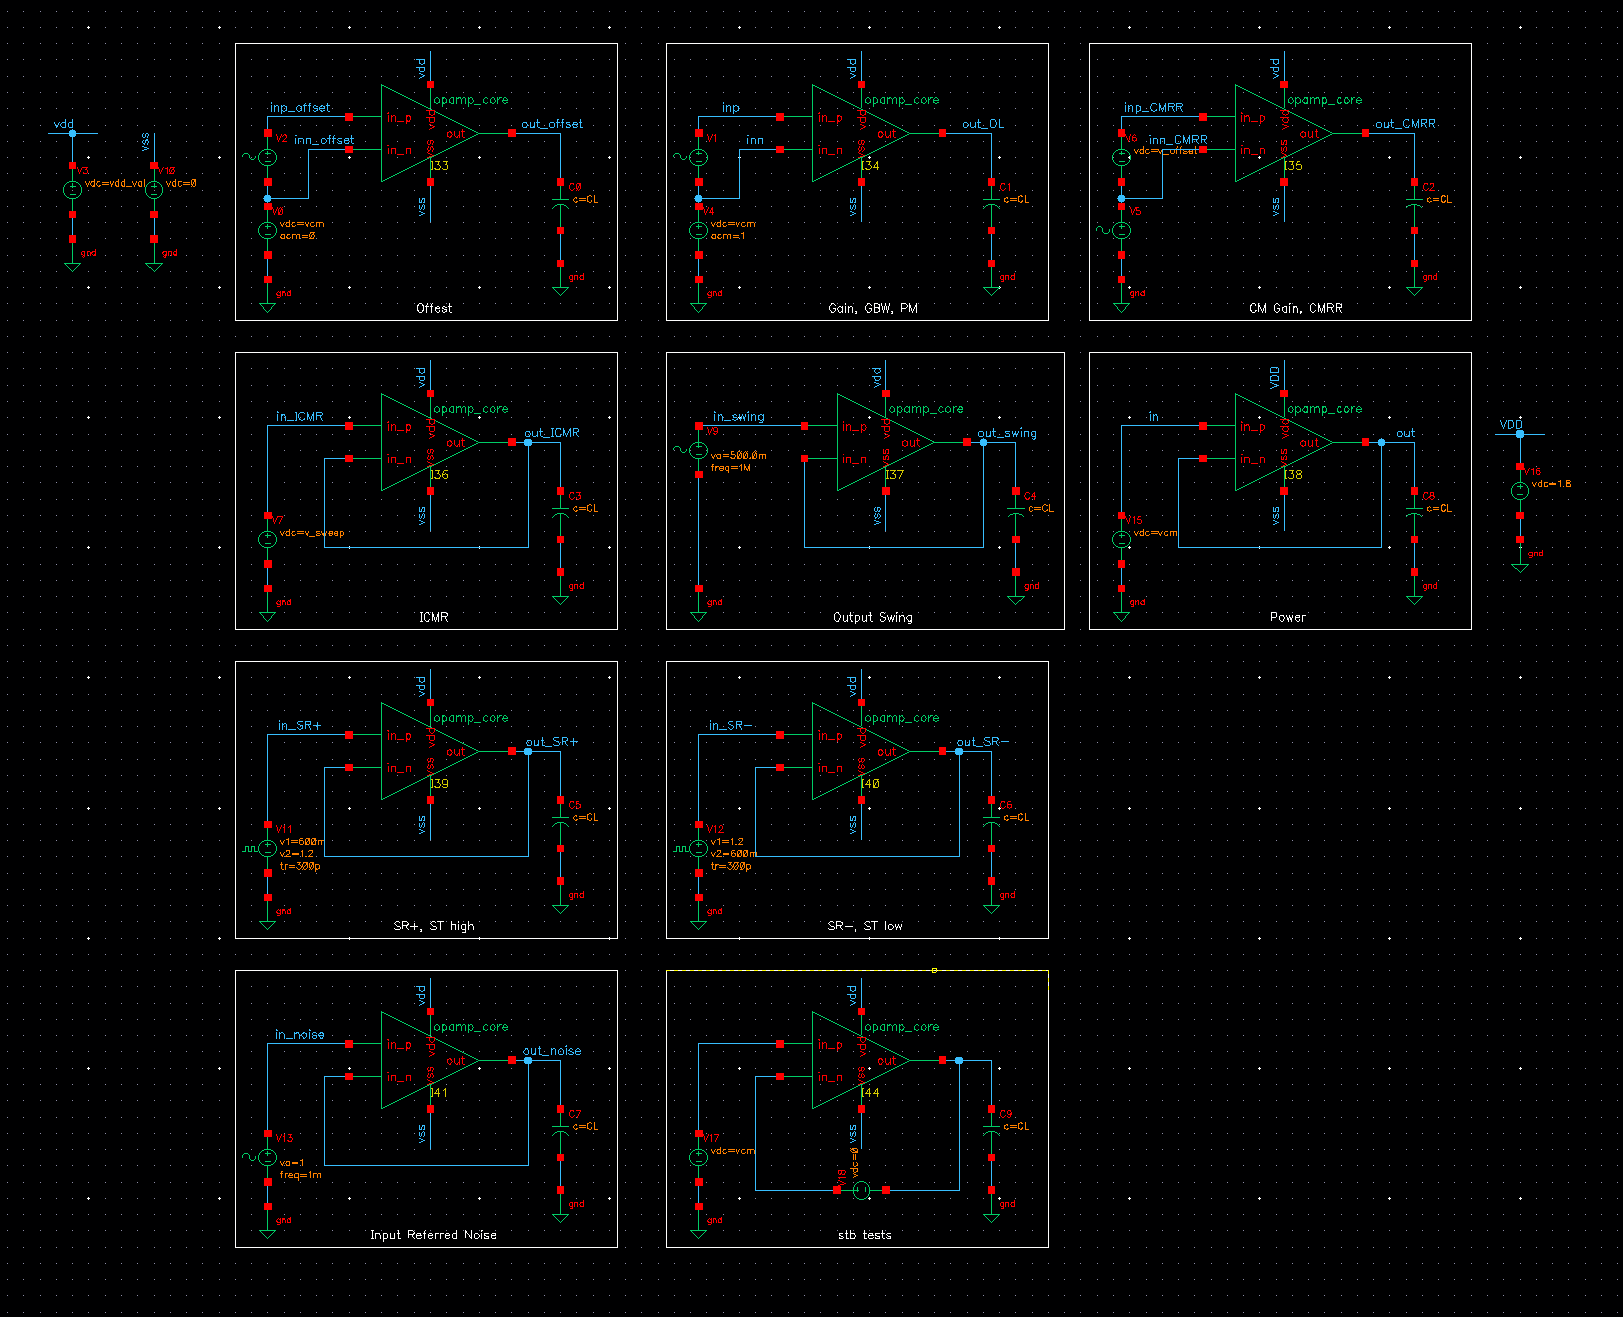
\includegraphics[width=\textwidth]{figures/opamp/testbench_final.png}
\caption{Schematic-level OPAMP testbenches for offset, AC/stability, CMRR, ICMR, output swing, power, slew/settling, and input noise. Each simulated output uses a \SI{2}{pF} load.}
\label{fig:testbench}
\end{figure}

The AC sweep covers \SI{1}{Hz}--\SI{1}{GHz} with 80 points per decade, while the noise sweep covers \SI{1}{Hz}--\SI{100}{MHz}; transient simulations run for \SI{1}{\micro s}. Slew and settling use \SI{0.6}{V}/\SI{1.2}{V} pulses with \SI{300}{ps} edges. The output-swing test uses a unity follower driven by \SI{0.9}{V} $\pm$ \SI{0.5}{V} at \SI{1}{MHz}.

\section{Nominal results}

Nominal simulations use TT/typical models at \SI{27}{\degreeCelsius}, \(\VDD=\SI{1.8}{V}\), \(\VCM=\SI{0.9}{V}\), and a \SI{2}{pF} load. The reported temperature is the exported simulation value.

% LAYOUT HANDOFF: Fill the Post-layout column from the extracted-view run and
% add a separate PEX pass/fail entry if the final table format is adjusted.
% Keep every schematic value unchanged. See ../../docs/verification.md.

\begin{table}[H]
\centering
\caption{Nominal OPAMP results with a \SI{2}{pF} load (course Table~2). Post-layout entries remain unavailable because no extracted-view simulation output was supplied.}
\label{tab:nominal-spec}
\small
\resizebox{\textwidth}{!}{%
\begin{tabular}{@{}llllll@{}}
\toprule
Metric & Requirement & Schematic nominal & Status & Post-layout & Simulation output \\
\midrule
DC gain & $>50$ dB & 79.93 dB & Pass & -- & ADE scalar \\
GBW & $\geq20$ MHz & 51.31 MHz & Pass & -- & ADE scalar \\
Phase margin & $\geq55^\circ$ & $61.97^\circ$ & Pass & -- & ADE scalar \\
CMRR & $>60$ dB & 68.53 dB & Pass & -- & ADE scalar \\
SR+ / SR$-$ & $\geq15/15$ V/\si{\micro s} & 35.17 / 27.43 V/\si{\micro s} & Pass & -- & transient scalars \\
Settling high / low (5\%) & $\leq500/500$ ns & 16.39 / 23.17 ns & Pass & -- & transient scalars \\
ICMR & 0.5--1.3 V & 0.8503 mV max. error & Pass & -- & clipped follower sweep \\
Output swing & 0.3--1.5 V & 0.4302--1.4006 V & Does not meet & -- & follower transient \\
Input offset & $\leq5$ mV abs. & $-0.4516$ mV & Pass & -- & ADE scalar \\
Noise at 20 kHz & $\leq55$ nV/$\sqrt{\mathrm{Hz}}$ & 32.78 nV/$\sqrt{\mathrm{Hz}}$ & Pass & -- & scalar and marker \\
Power & $\leq0.6$ mW & 0.3113 mW & Pass & -- & ADE scalar \\
Area & report value & n/a & n/a & -- & no scaled layout export \\
\bottomrule
\end{tabular}}
\end{table}

For the ICMR check, we configured the OPAMP as a unity-gain follower and swept the non-inverting input from \SI{0}{V} to \SI{1.8}{V}. The ADE expression clips the waveform to the required \SIrange{0.5}{1.3}{V} interval before taking the maximum error:
\begin{equation}
\varepsilon_{\mathrm{ICMR,max}}
=\max_{0.5\,\mathrm{V}\leq V_{\mathrm{in}}\leq1.3\,\mathrm{V}}
\left|V_{\mathrm{out}}(V_{\mathrm{in}})-V_{\mathrm{in}}\right|
=\SI{850.3}{\micro V}.
\end{equation}
The resulting \SI{0.8503}{mV} maximum error is well below the \SI{50}{mV} limit. This verifies the specified ICMR interval with the stated follower-error criterion; the wider \SIrange{0}{1.8}{V} sweep is only the test range and is not reported as the ICMR.

The simulated output swing is approximately \SIrange{0.430}{1.401}{V}, with raw limits of \SI{0.430203}{V} and \SI{1.40056}{V}. This does not cover the full specified \SIrange{0.3}{1.5}{V} range. We retained the circuit because earlier changes reduced the available margins in stability, slew rate, CMRR, noise, or power. The limitation caused no failure in the available PGA corner or Monte Carlo runs under their applied stimuli, although those runs do not turn the swing result into a specification pass.

The input-noise scalar is \SI{32.7766}{nV}/$\sqrt{\mathrm{Hz}}$. At \SI{20}{kHz}, the waveform marker reads \SI{32.8072}{nV}/$\sqrt{\mathrm{Hz}}$. The \SI{0.0306}{nV}/$\sqrt{\mathrm{Hz}}$ difference is consistent with display and sampling precision and supports the rounded \SI{32.78}{nV}/$\sqrt{\mathrm{Hz}}$ result in Tables~\ref{tab:nominal-spec} and \ref{tab:corners}.

% TODO(figure readability): Replace the nominal overview with larger individual crops if new exports are available. The present composite documents the waveform set, while exact values are taken from the tables and scalar outputs.
\begin{figure}[p]
\centering
\textbf{(a) Nominal overview}\par\smallskip
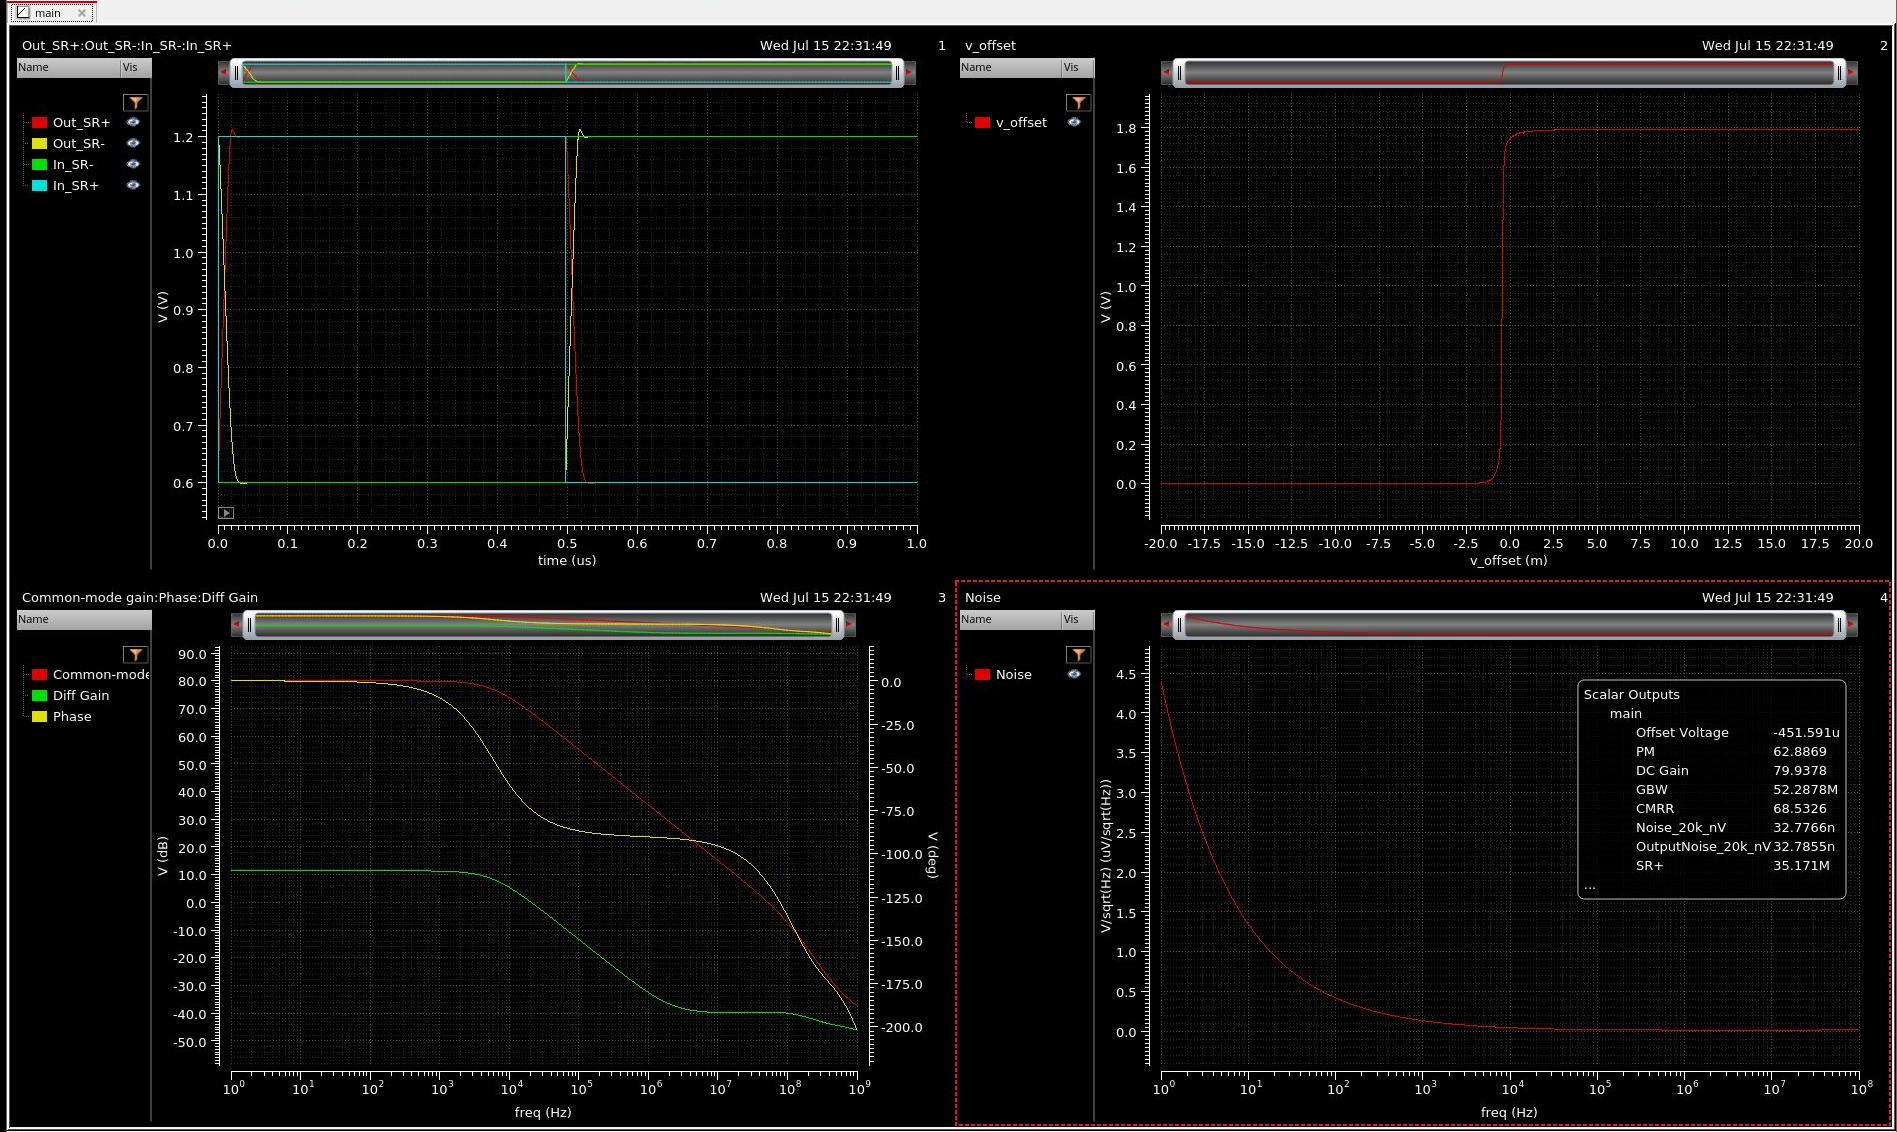
\includegraphics[width=0.66\textwidth]{figures/opamp/nominal_overview.png}

\smallskip
\textbf{(b) ICMR criterion and result}\par\smallskip
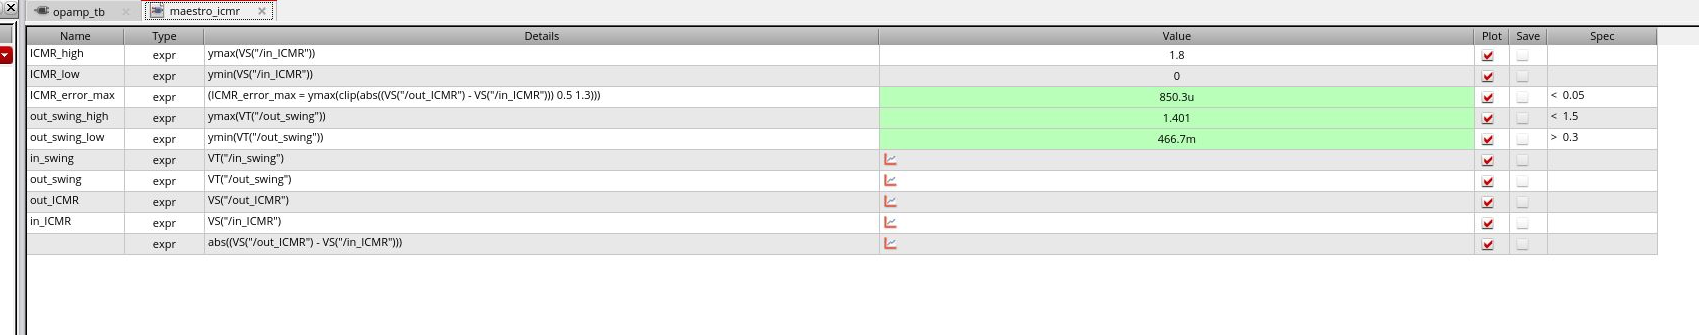
\includegraphics[width=0.96\textwidth,trim=0 225 470 0,clip]{figures/opamp/icmr_expression.png}

\smallskip
\begin{minipage}[t]{0.31\textwidth}
\centering
\textbf{(c) Output swing}\par\smallskip
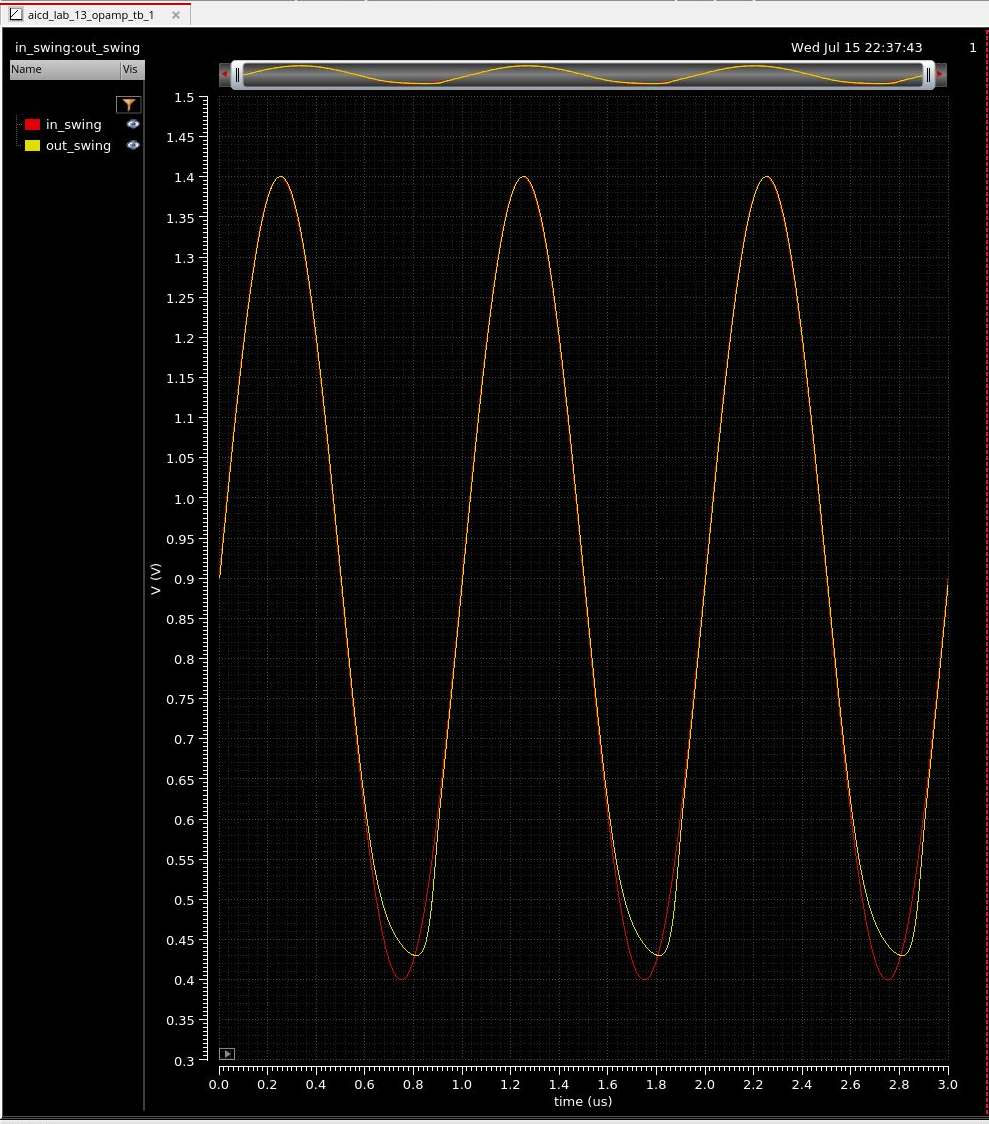
\includegraphics[width=\linewidth]{figures/opamp/output_swing.png}
\end{minipage}\hspace{0.035\textwidth}
\begin{minipage}[t]{0.41\textwidth}
\centering
\textbf{(d) Input noise at \SI{20}{kHz}}\par\smallskip
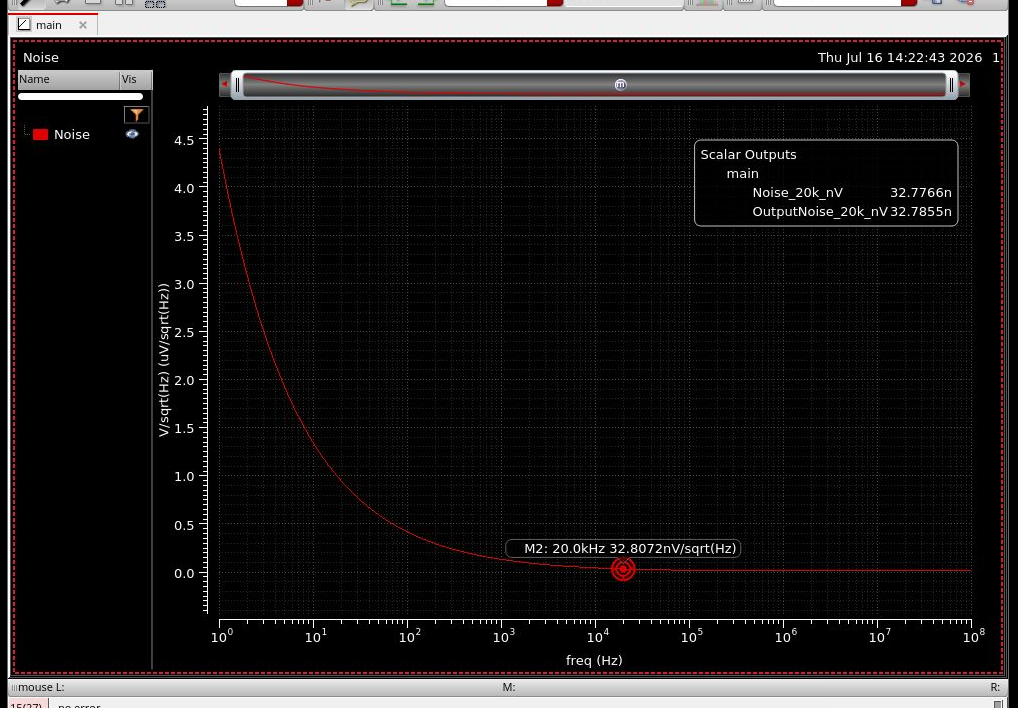
\includegraphics[width=\linewidth]{figures/opamp/noise_20k.png}
\end{minipage}
\caption{Nominal OPAMP simulations: (a) response overview, (b) clipped ICMR follower-error expression and scalar result, (c) output-swing transient, and (d) input-noise spectrum with a \SI{20}{kHz} marker. Exact values are reported in Table~\ref{tab:nominal-spec}.}
\label{fig:opamp-key-plots}
\end{figure}

\section{PVT-corner results}

The PVT sweep combines two MIM sections, two resistor sections, four device/process sections, two temperatures (\SI{-25}{\degreeCelsius}, \SI{85}{\degreeCelsius}), and two supplies (\SI{1.62}{V}, \SI{1.98}{V}):
\begin{equation}
N_{\mathrm{corner}}=2\times2\times4\times2\times2=64.
\end{equation}

Every one of the 12 output expressions included in the export is marked \texttt{pass}. Table~\ref{tab:corners} therefore reports 64/64 directly from the raw CSV. ICMR and output swing are not part of this corner export; the all-pass statement does not cover them.

% LAYOUT HANDOFF: For the final report, write each PEX value first and the
% schematic value in parentheses. Report the PEX and schematic pass counts
% separately, e.g. 64 (64)/64. Do not extend the claim to ICMR or swing unless
% those expressions are explicitly added to the extracted-view sweep.

\begin{table}[H]
\centering
\caption{PVT-corner summary with a \SI{2}{pF} load (course Table~3).}
\label{tab:corners}
\small
\resizebox{\textwidth}{!}{%
\begin{tabular}{@{}lrrrrrl@{}}
\toprule
Metric & Requirement & Nominal & Minimum & Maximum & Passed/total & Limiting corner \\
\midrule
DC gain (dB) & $>50$ & 79.93 & 76.32 & 82.76 & 64/64 & C9, minimum \\
GBW (MHz) & $\geq20$ & 51.31 & 32.28 & 72.94 & 64/64 & C57, minimum \\
Phase margin ($^\circ$) & $\geq55$ & 61.97 & 59.57 & 68.81 & 64/64 & C4, minimum \\
CMRR (dB) & $>60$ & 68.53 & 61.54 & 74.50 & 64/64 & C26, minimum \\
SR+ (V/\si{\micro s}) & $\geq15$ & 35.17 & 22.34 & 49.14 & 64/64 & C41, minimum \\
SR$-$ (V/\si{\micro s}) & $\geq15$ & 27.43 & 16.04 & 34.90 & 64/64 & C56, minimum \\
Settling high (ns) & $\leq500$ & 16.39 & 11.77 & 26.36 & 64/64 & C41, maximum \\
Settling low (ns) & $\leq500$ & 23.17 & 18.11 & 41.74 & 64/64 & C56, maximum \\
Offset (mV) & $\lvert\cdot\rvert\leq5$ & $-0.4516$ & $-0.7204$ & $-0.2660$ & 64/64 & C41, max. absolute \\
Noise (nV/$\sqrt{\mathrm{Hz}}$) & $\leq55$ & 32.78 & 29.17 & 45.73 & 64/64 & C49, maximum \\
Power (\si{\micro W}) & $\leq600$ & 311.3 & 266.3 & 367.8 & 64/64 & C9, maximum \\
\bottomrule
\end{tabular}}
\end{table}

The closest numeric limits are SR$-$ with \SI{1.04}{V/\micro s} headroom, CMRR with \SI{1.54}{dB}, and phase margin with \SI{4.57}{\degree}. The worst noise value still has \SI{9.27}{nV}/$\sqrt{\mathrm{Hz}}$ of headroom. The raw export identifies C56 as the slow-resistor/slow-process, \SI{-25}{\degreeCelsius}, \SI{1.62}{V} point; C26 limits CMRR, and C4 limits phase margin.

\section{Schematic Monte Carlo analysis}

The Monte Carlo analysis uses variation \texttt{All}, 1000 points, standard random sampling, seed 12345, and first point 1. Separate transient, offset, and stability tests provide 1000 samples for each reported metric.

% LAYOUT HANDOFF: Add the 1000-point extracted-view statistics in the form
% PEX (schematic), including yield. Do not replace the 972/1000 schematic
% offset yield. See ../../docs/verification.md.

\begin{table}[H]
\centering
\caption{OPAMP Monte Carlo summary, 1000 samples per test (course Table~4).}
\label{tab:mc}
\small
\resizebox{\textwidth}{!}{%
\begin{tabular}{@{}lrrrrrrl@{}}
\toprule
Metric & Minimum & Maximum & Mean & $\sigma$ & Yield & Errors & Status \\
\midrule
DC gain (dB) & 79.09 & 80.75 & 79.93 & 0.2452 & 1000/1000 & 0 & Pass \\
GBW (MHz) & 42.09 & 63.05 & 51.42 & 3.250 & 1000/1000 & 0 & Pass \\
Phase margin ($^\circ$) & 56.28 & 66.40 & 61.93 & 1.479 & 1000/1000 & 0 & Pass \\
SR+ (V/\si{\micro s}) & 27.06 & 44.66 & 35.16 & 2.742 & 1000/1000 & 0 & Pass \\
SR$-$ (V/\si{\micro s}) & 21.82 & 35.37 & 27.43 & 2.072 & 1000/1000 & 0 & Pass \\
Settling high (ns) & 12.94 & 21.31 & 16.48 & 1.282 & 1000/1000 & 0 & Pass \\
Settling low (ns) & 17.94 & 29.65 & 23.31 & 1.786 & 1000/1000 & 0 & Pass \\
Offset (mV) & $-7.447$ & 5.518 & $-0.4735$ & 2.212 & 972/1000 & 0 & 97.2\% \\
\bottomrule
\end{tabular}}
\end{table}

Offset is the only reported metric with less than 100\% yield. Its mean is \SI{-0.474}{mV}, and 28 of 1000 samples exceed the \SI{5}{mV} absolute limit, giving 972/1000.

\begin{figure}[htbp]
\centering
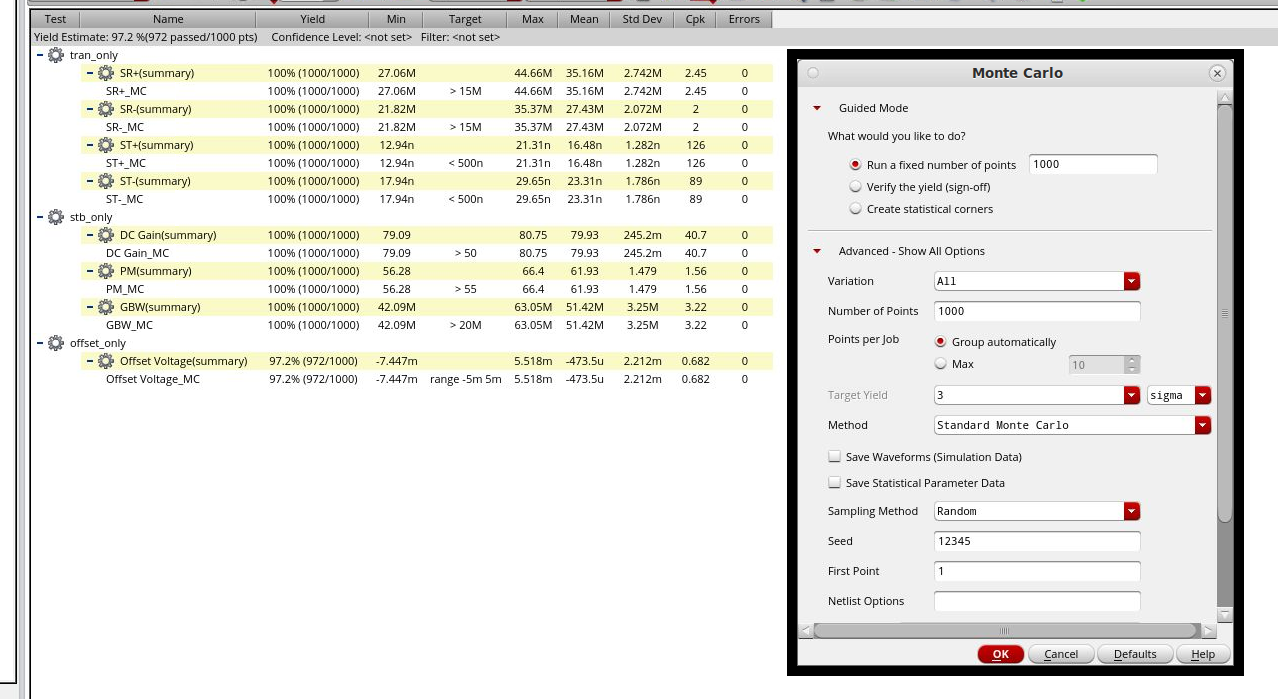
\includegraphics[width=\textwidth]{figures/opamp/mc_summary.png}
\caption{ADE Monte Carlo summary and sampling setup for variation \texttt{All}, 1000 samples per test, random sampling, and seed 12345.}
\label{fig:mc-summary}
\end{figure}

\chapter{Programmable-Gain Amplifier and Active Low-Pass Filter}

\section{Circuit hierarchy}

The signal path places a programmable inverting stage before a unity-gain active LPF. Both stages reuse the OPAMP of Chapter~2 without changing its intended effective sizing, bias function, or compensation. Nominal simulations use \(\VDD=\SI{1.8}{V}\), \(\VCM=\SI{0.9}{V}\), and a \SI{2}{pF} load.

The schematic is now split into smaller cells. The \texttt{PGA\_core} cell contains the input resistor, OPAMP, segmented feedback string, and eight transmission-gate taps. The LPF is a separate cell with its own OPAMP, equal input and feedback resistor strings, enable switch, and capacitor. A wrapper connects the behavioral Controller outputs to the PGA core. This separation keeps the analog path readable and makes the testbench less dependent on one large top-level schematic.

\begin{figure}[p]
\centering
\textbf{(a) PGA core}\par\smallskip
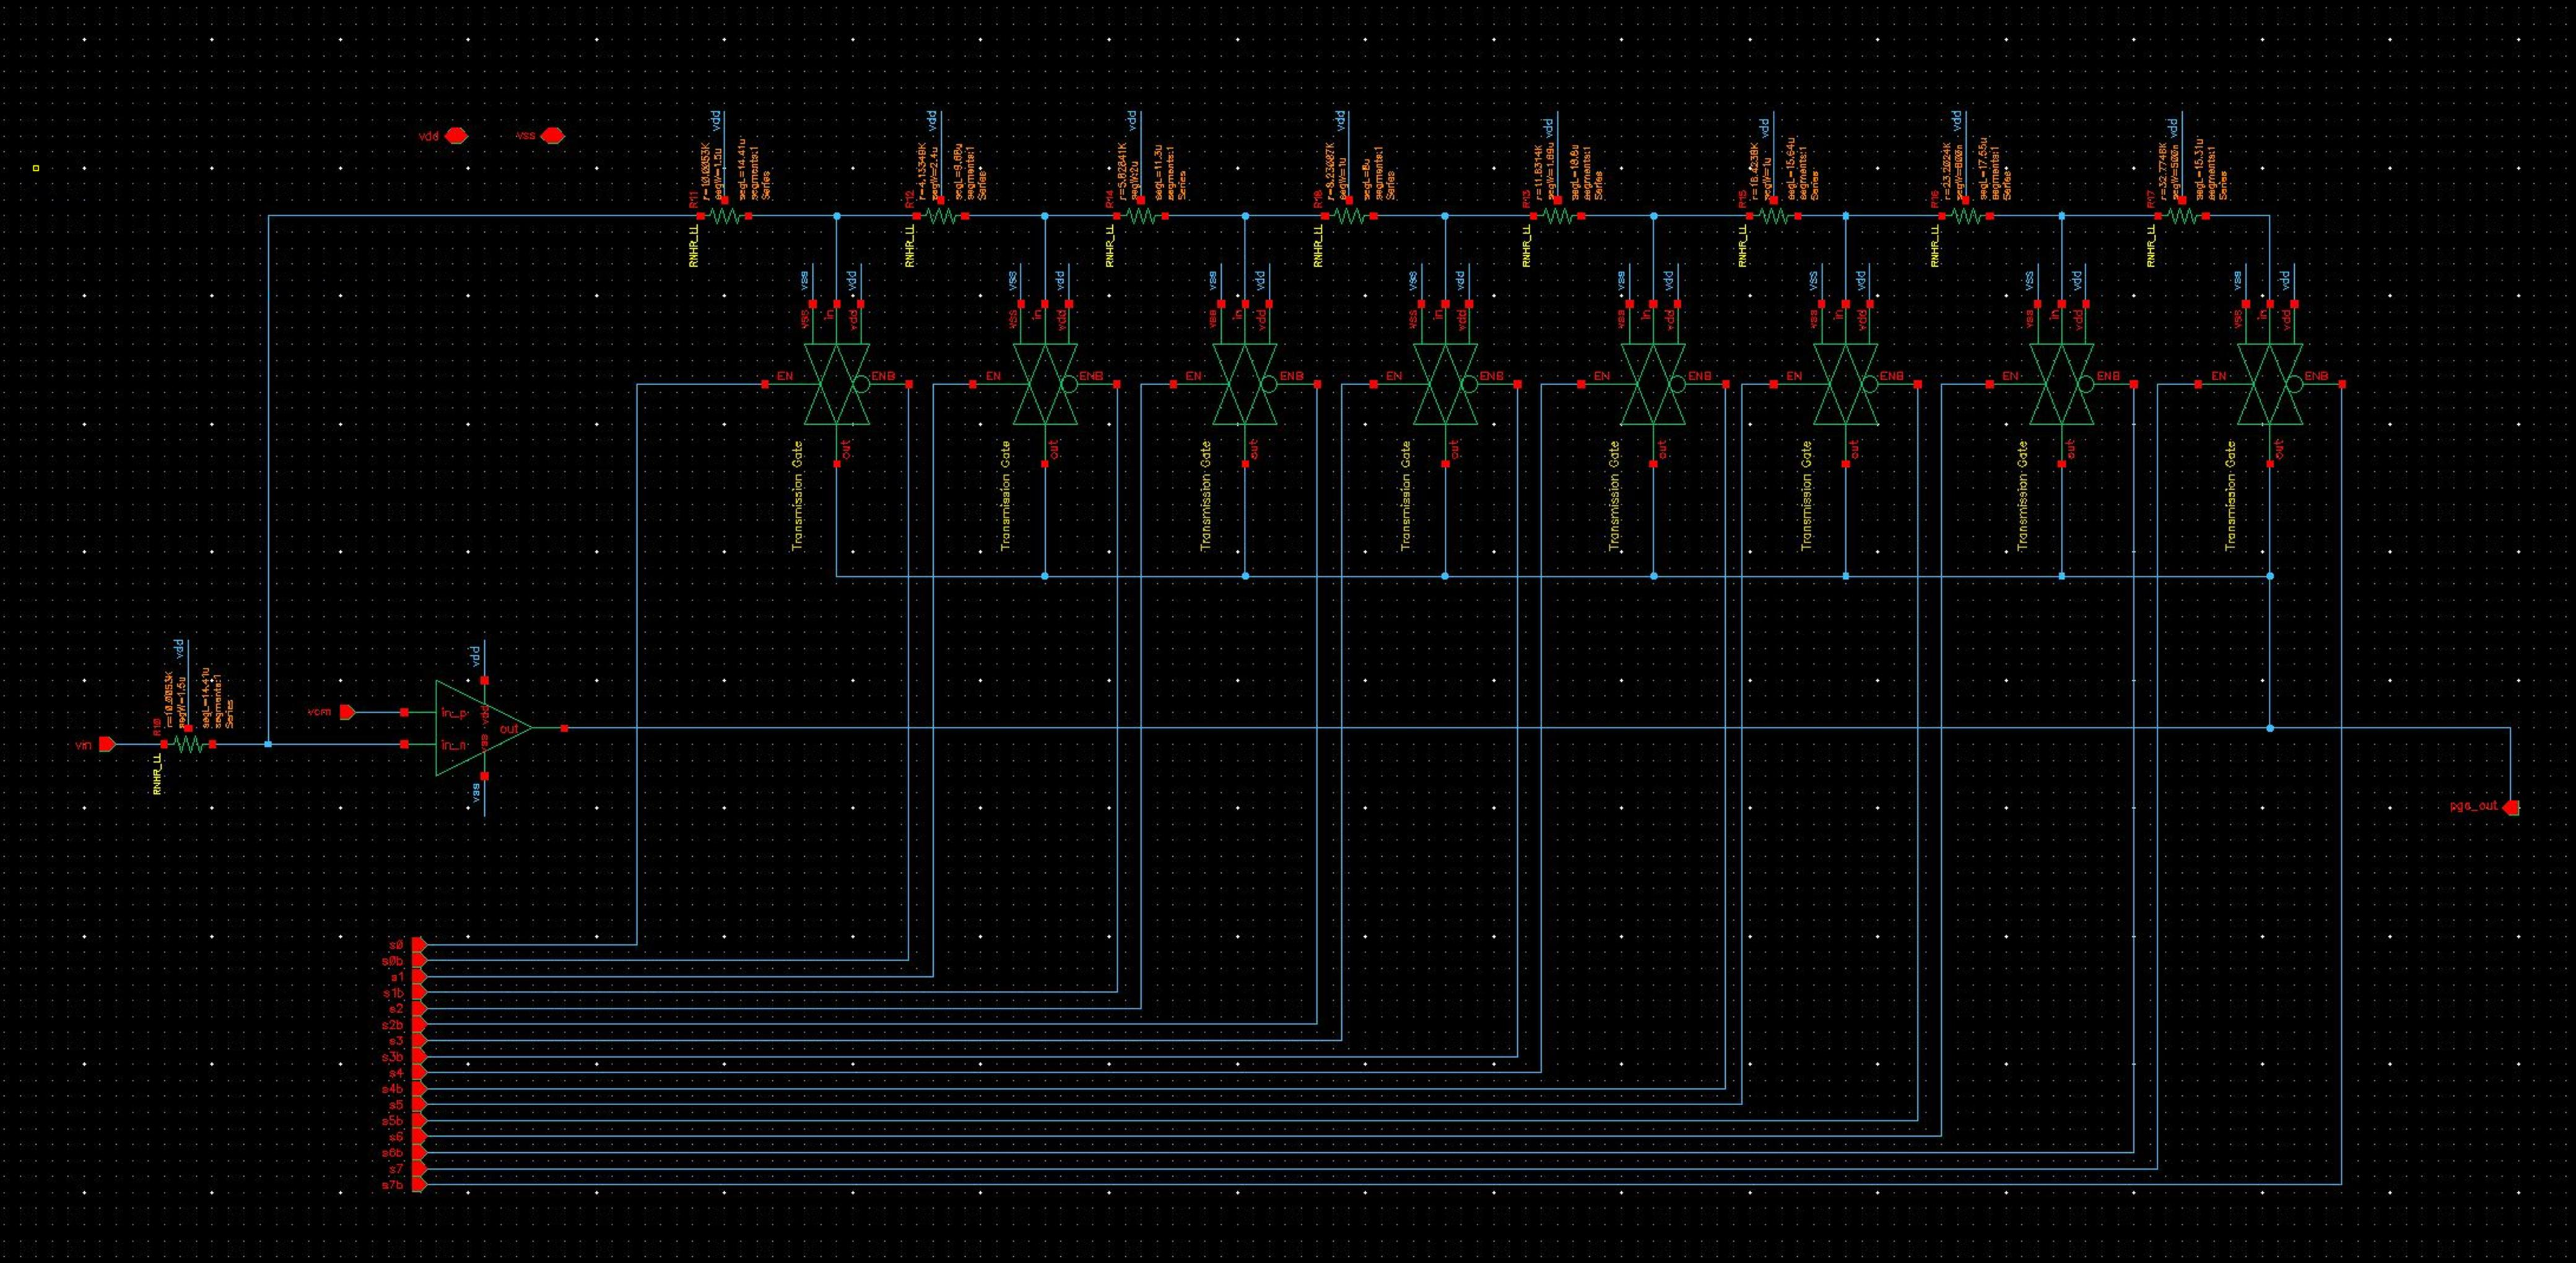
\includegraphics[width=0.96\textwidth]{figures/pga/pga_core.jpeg}

\medskip
\textbf{(b) Active low-pass filter}\par\smallskip
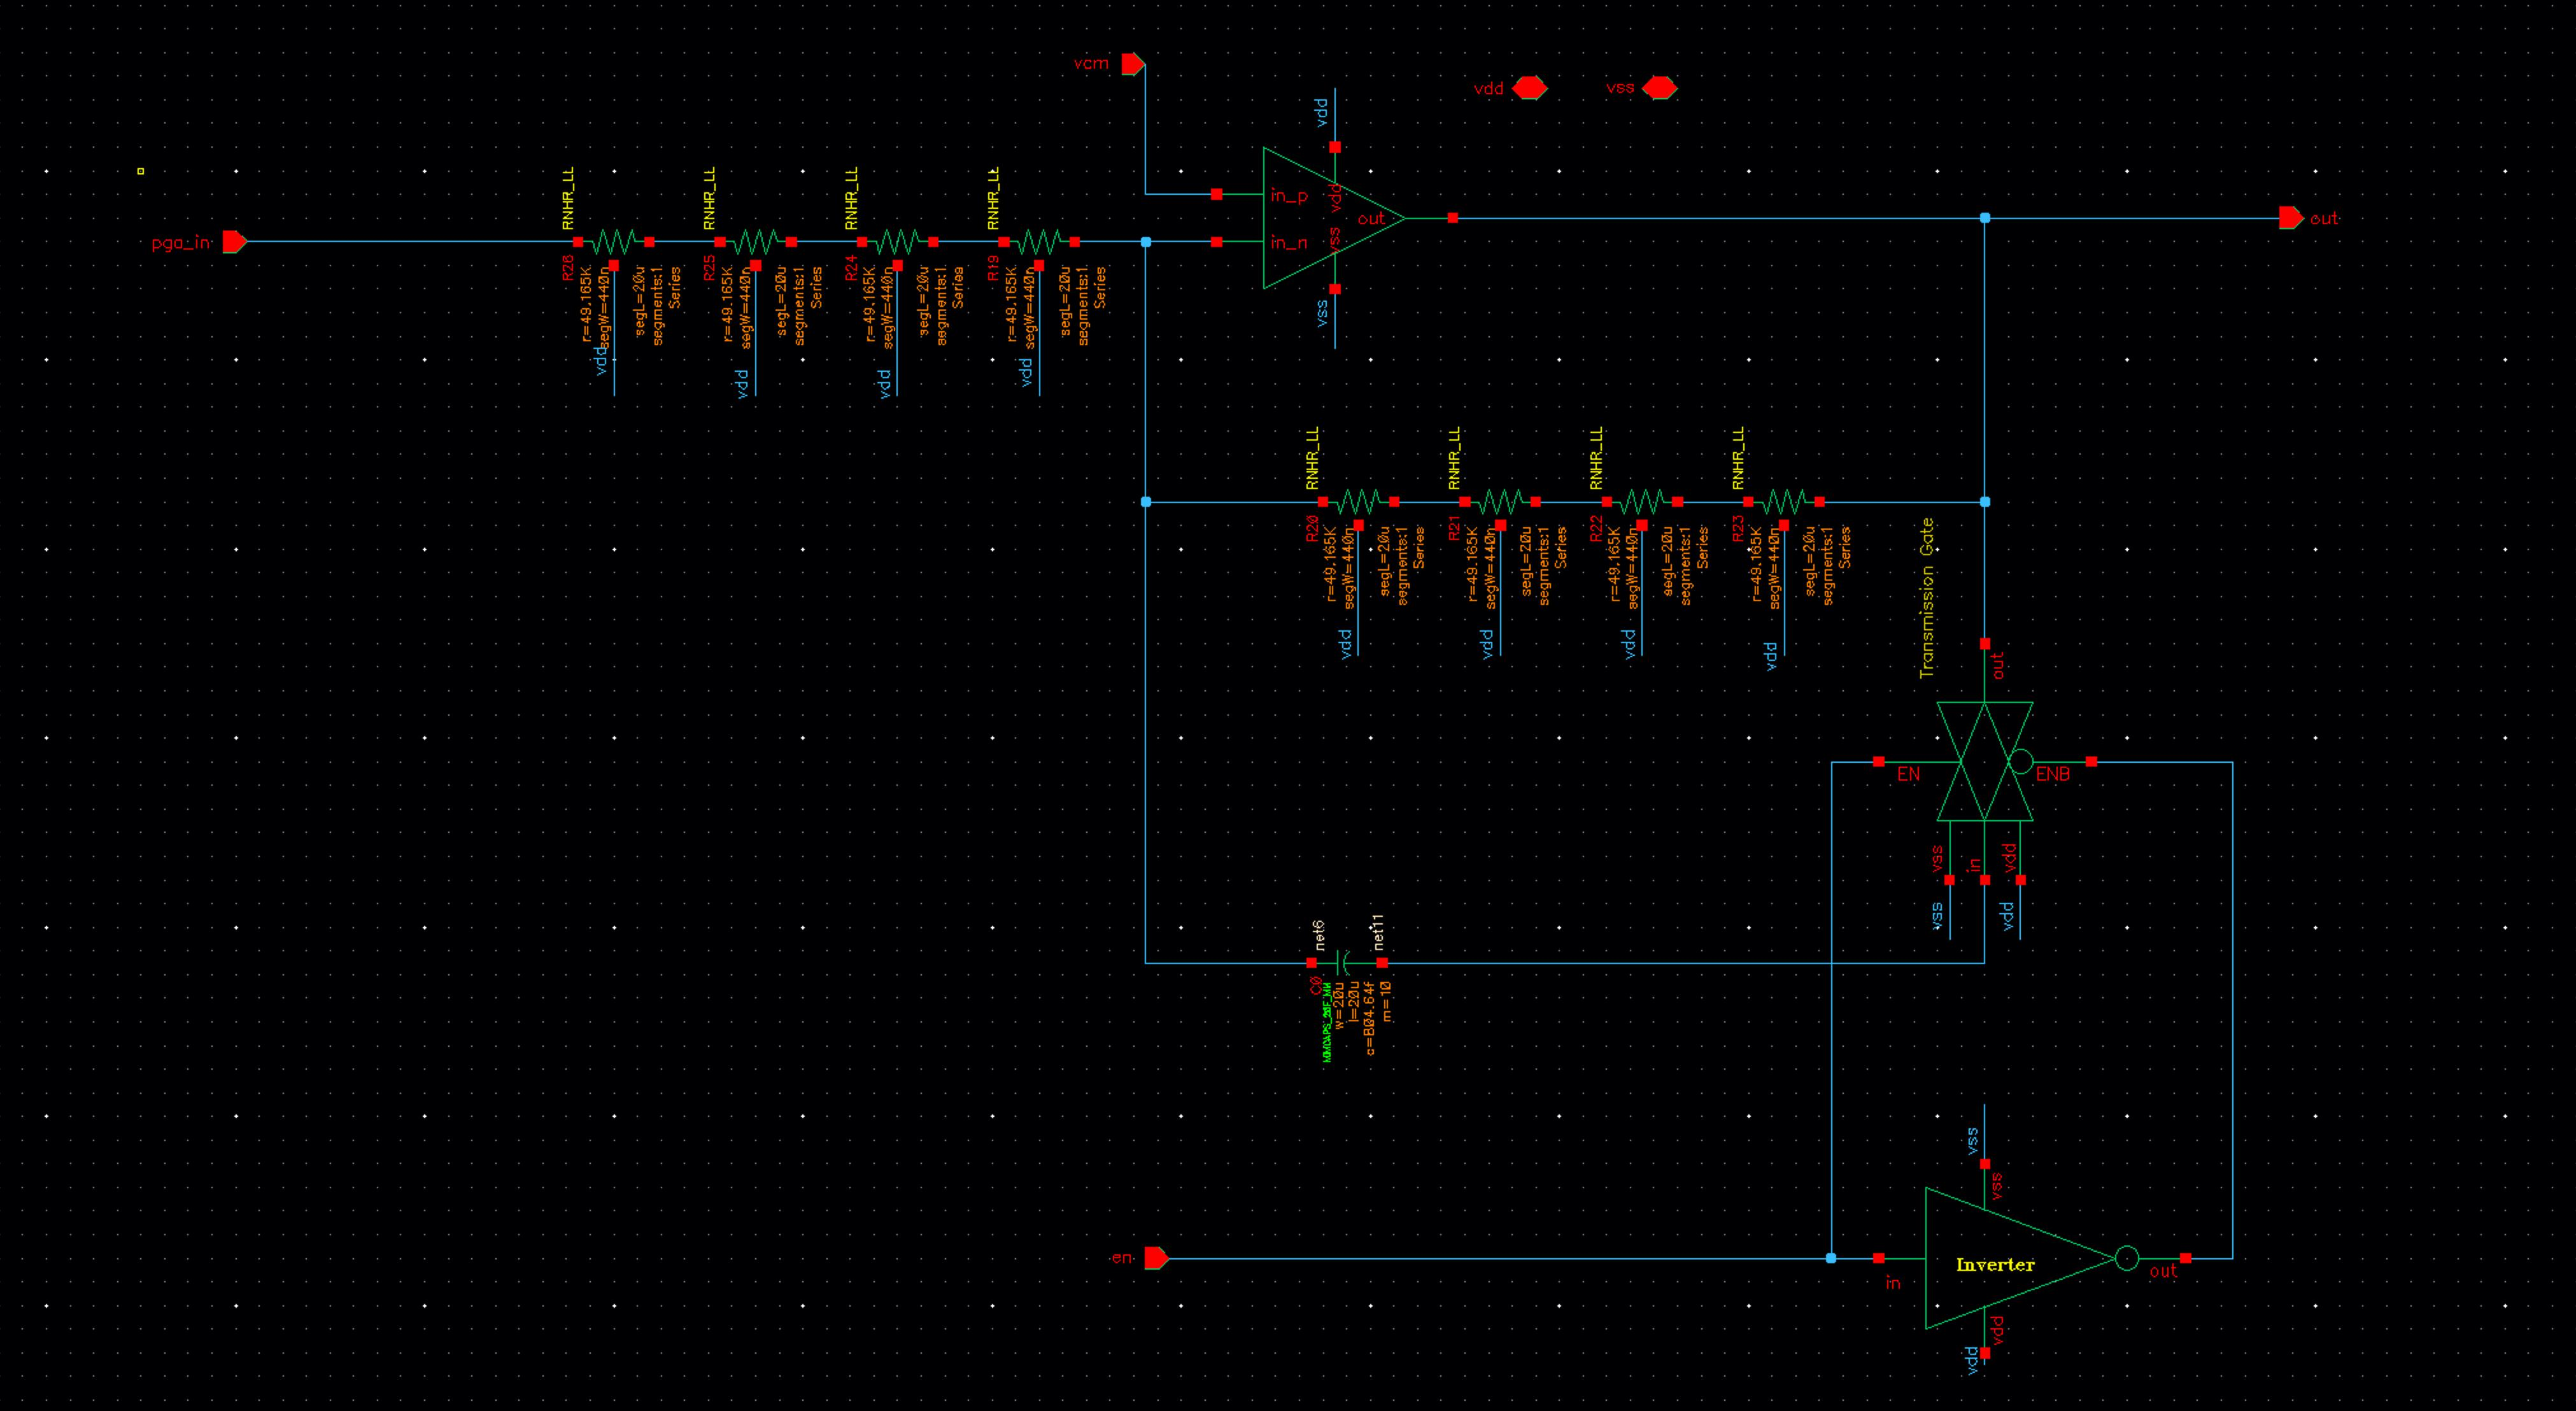
\includegraphics[width=0.90\textwidth]{figures/pga/lpf_schematic.jpeg}
\caption{Updated component schematics. The PGA core contains the programmable feedback network and its OPAMP; the LPF remains a separate enabled unity-gain stage.}
\label{fig:pga-component-schematics}
\end{figure}

The wrapper accepts \texttt{b0}--\texttt{b2}, \texttt{vin}, and \texttt{vcm}. The Controller generates eight one-hot outputs and their complements, and the wrapper routes them directly to the corresponding PGA-core switches. The PGA output remains available as \texttt{pga\_out}; the LPF is instantiated separately in the testbench so that the PGA and filter responses can still be measured independently.

\begin{figure}[p]
\centering
\textbf{(a) Controller and PGA wrapper}\par\smallskip
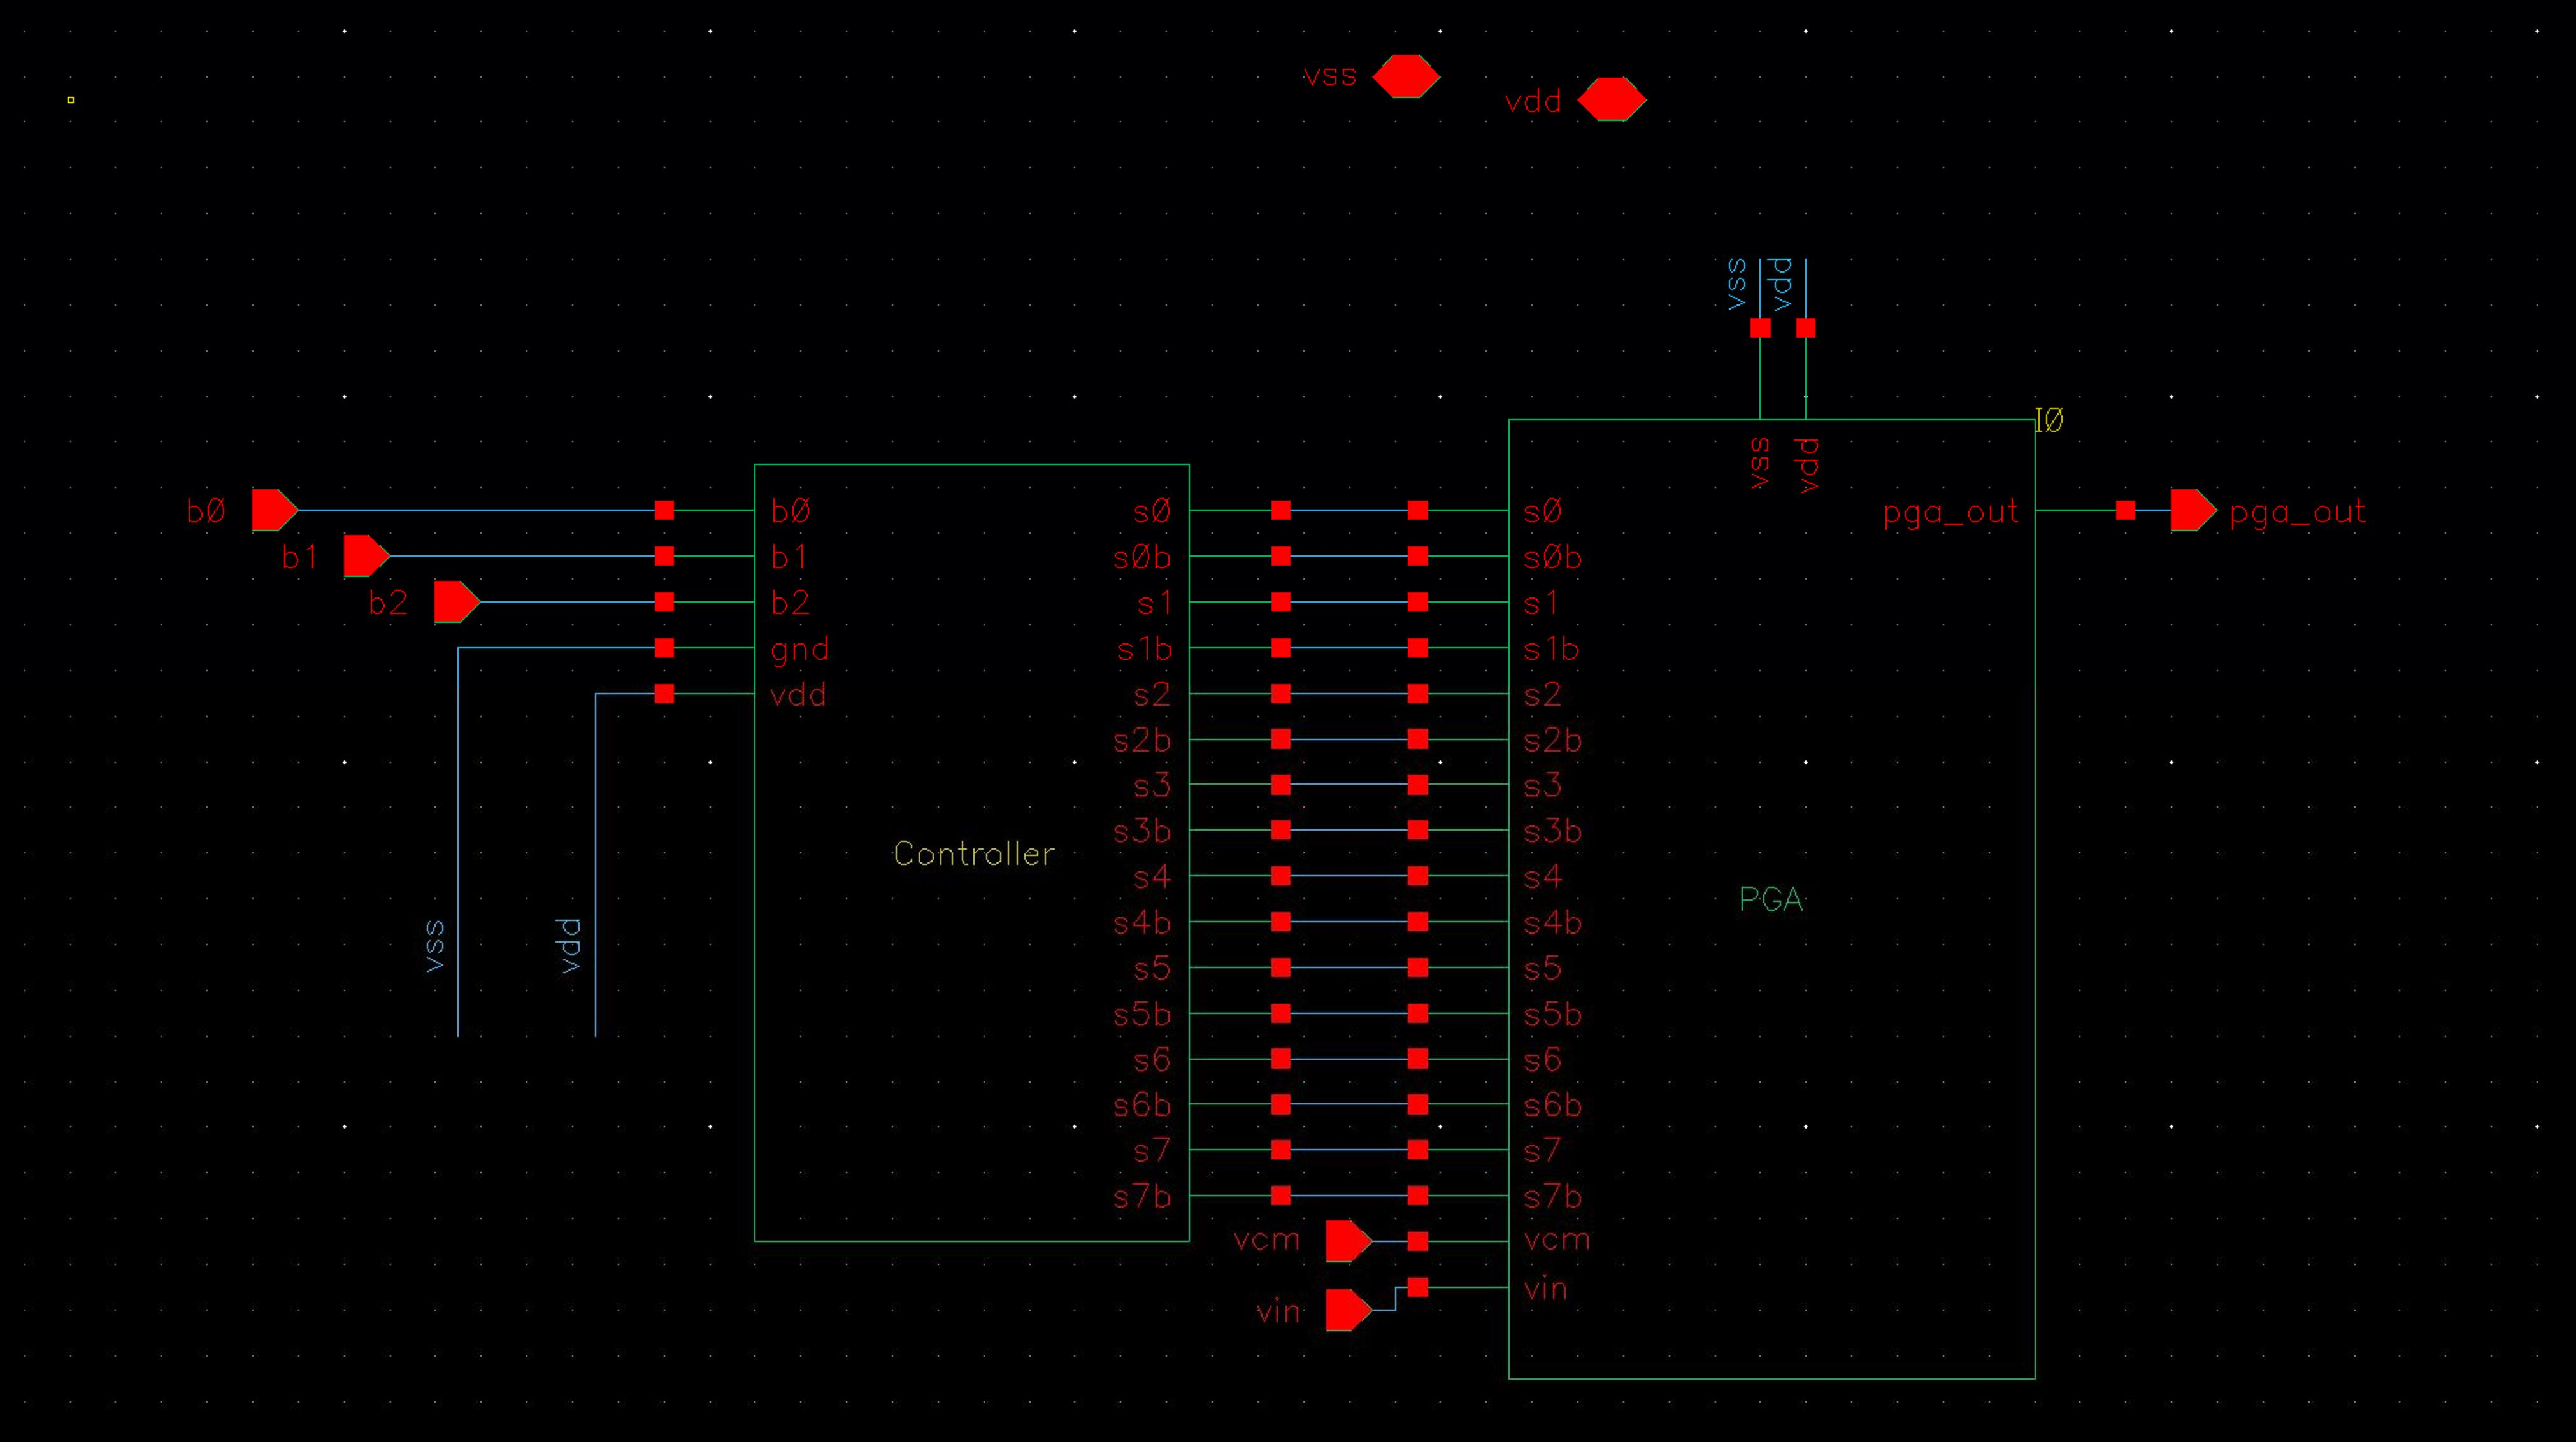
\includegraphics[width=0.72\textwidth]{figures/pga/pga_wrapper.jpeg}

\smallskip
\textbf{(b) Updated PGA and LPF testbench}\par\smallskip
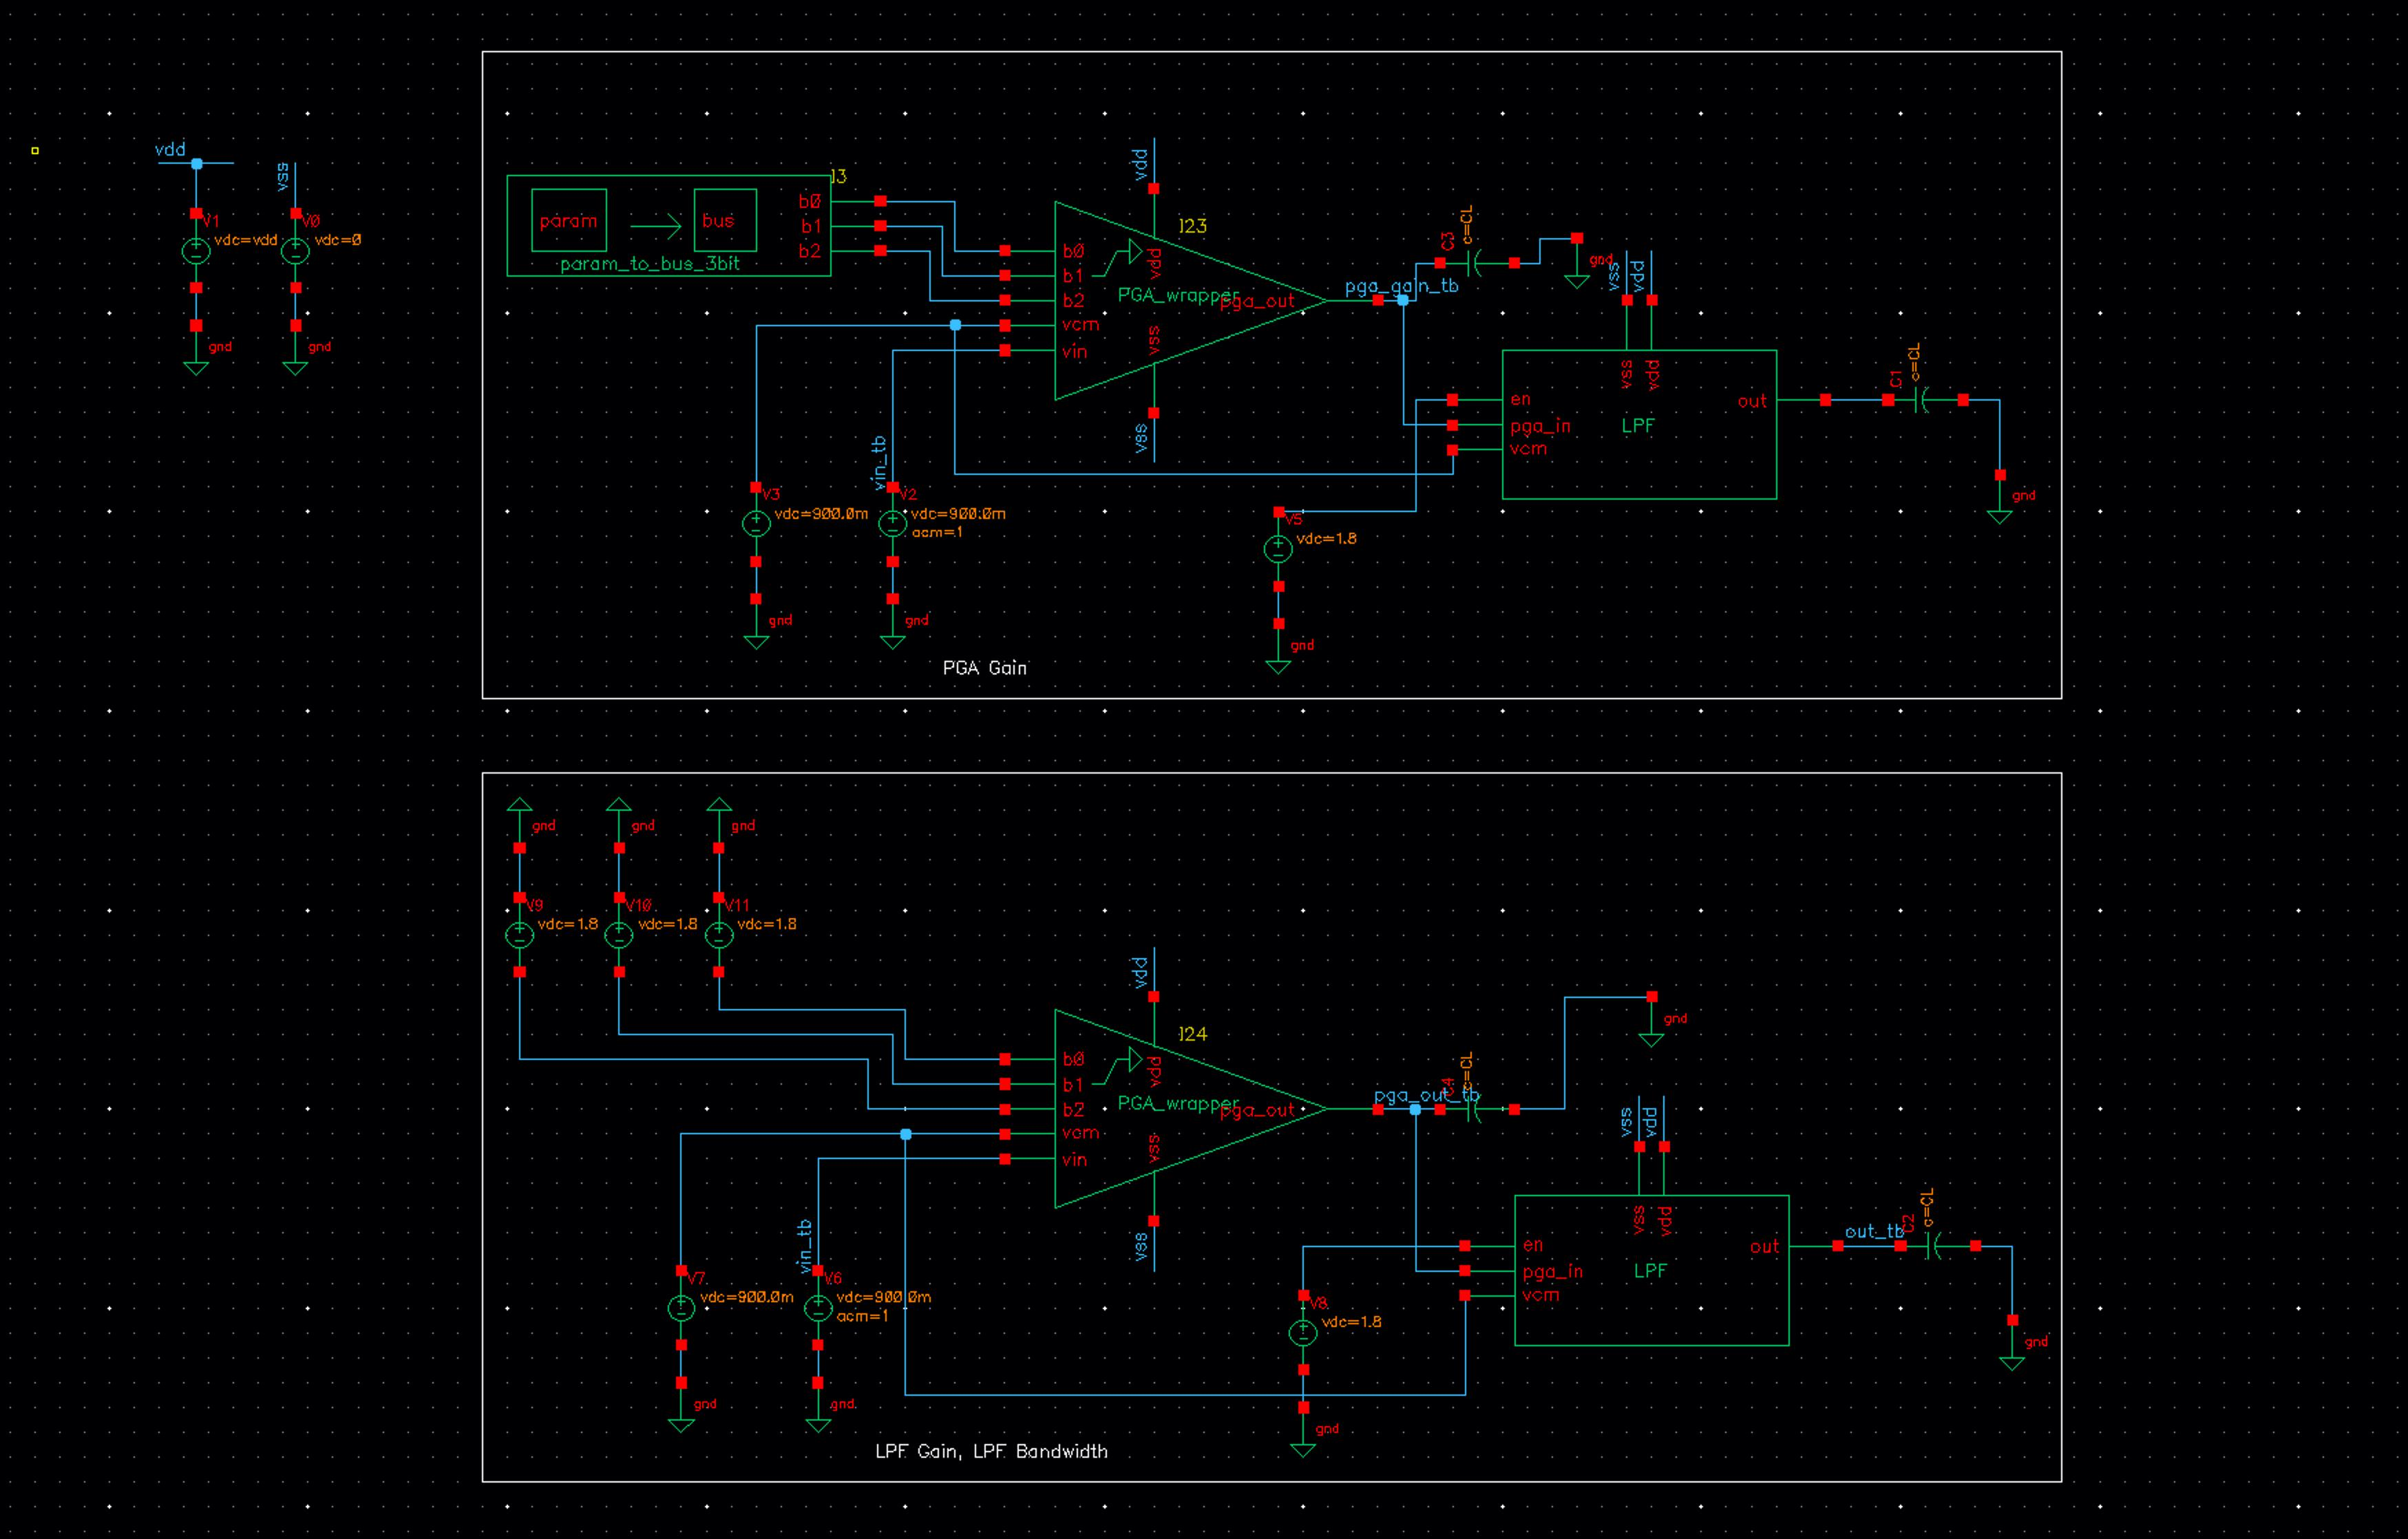
\includegraphics[width=0.88\textwidth]{figures/pga/pga_testbench_modular.jpeg}
\caption{Updated hierarchy and testbench. The upper test region drives the wrapper from a parameter-to-bus block for the gain-code sweep; the lower region uses explicit code sources for the LPF gain and bandwidth checks.}
\label{fig:pga-wrapper-testbench}
\end{figure}

These captures document the new hierarchy and wiring. No new ADE scalar, corner, or Monte Carlo export tied specifically to this refactoring was supplied, so the numerical tables in this chapter remain the verified schematic baseline.

\section{PGA feedback network and control}

For an ideal inverting stage referenced to \(\VCM\),
\begin{align}
\frac{V_{\mathrm{out}}-\VCM}{V_{\mathrm{in}}-\VCM}
&=-\frac{R_2}{R_1}, \\
G_{\mathrm{dB}}
&=20\log_{10}\!\left(\frac{R_2}{R_1}\right), \\
R_2
&=R_1\,10^{G_{\mathrm{dB}}/20}.
\end{align}
We set the target input resistance to \SI{10}{k\ohm}; the implemented RNHR value is approximately \SI{10.0051}{k\ohm}. Table~\ref{tab:pga-resistors} shows that the cumulative feedback string follows the eight 3 dB targets closely before switch and finite-loop effects.

\begin{table}[htbp]
\centering
\caption{Implemented cumulative PGA feedback values.}
\label{tab:pga-resistors}
\footnotesize
\begin{tabular}{@{}lrrr@{}}
\toprule
Code & Target (dB) & Cumulative $R_2$ (k$\Omega$) & Passive gain (dB) \\
\midrule
000 & 0  & 10.00530  & 0.00017 \\
001 & 3  & 14.13878  & 3.00381 \\
010 & 6  & 19.96719  & 6.00191 \\
011 & 9  & 28.19806  & 8.99996 \\
100 & 12 & 39.82946  & 11.99966 \\
101 & 15 & 56.25326  & 14.99853 \\
110 & 18 & 79.45566  & 17.99807 \\
111 & 21 & 112.23026 & 20.99777 \\
\bottomrule
\end{tabular}
\end{table}

Each feedback tap uses a CMOS transmission gate with a \texttt{P\_25\_LL} device of \SI{50}{\micro m}/\SI{240}{nm} and an \texttt{N\_25\_LL} device of \SI{25}{\micro m}/\SI{240}{nm}. With the switch in series with \SI{100}{k\ohm}, we swept the input from \SI{0.3}{V} to \SI{1.5}{V} and evaluated the switch resistance as
\begin{equation}
R_{\mathrm{sw}}(V)=\left|\frac{V_{\mathrm{in}}-V_{\mathrm{out}}}{I_{\mathrm{sw}}}\right|.
\end{equation}
The worst measured values are \(\Ron=\SI{232.1}{\ohm}\) and \(\Roff=\SI{38.81}{\giga\ohm}\). The finite \(\Ron\) is small relative to \SI{10}{k\ohm}, but its relative gain error is largest at code 000.

The behavioral Verilog-A controller decodes the three-bit input into eight one-hot signals and their complements, with \texttt{vth\_ratio=0.5}, \texttt{td=0}, and \texttt{tr=tf=1 ns}. Sweeping all eight gain codes through the complete PGA testbench verifies the static decode path together with the MUX and feedback network.

% TODO(figure readability): Replace the transmission-gate screenshot with a larger resistance crop if available. The exact worst-case values are reported in the text because the on-resistance is compressed by the linear GOhm-scale axis.
\begin{figure}[htbp]
\centering
\begin{minipage}[t]{0.47\textwidth}
\centering
\textbf{(a) Nominal gain versus code}\par\smallskip
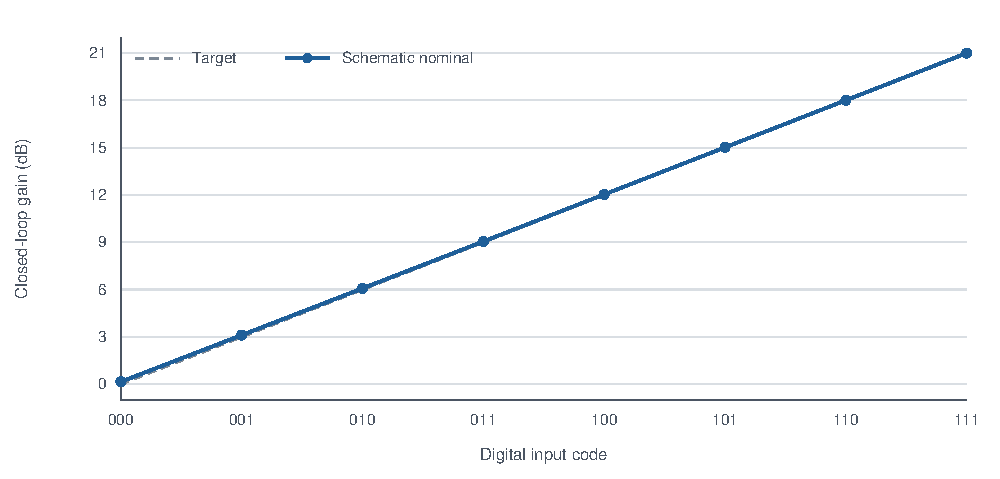
\includegraphics[width=\linewidth]{figures/pga/gain_vs_code.pdf}
\end{minipage}\hfill
\begin{minipage}[t]{0.47\textwidth}
\centering
\textbf{(b) TG on/off resistance}\par\smallskip
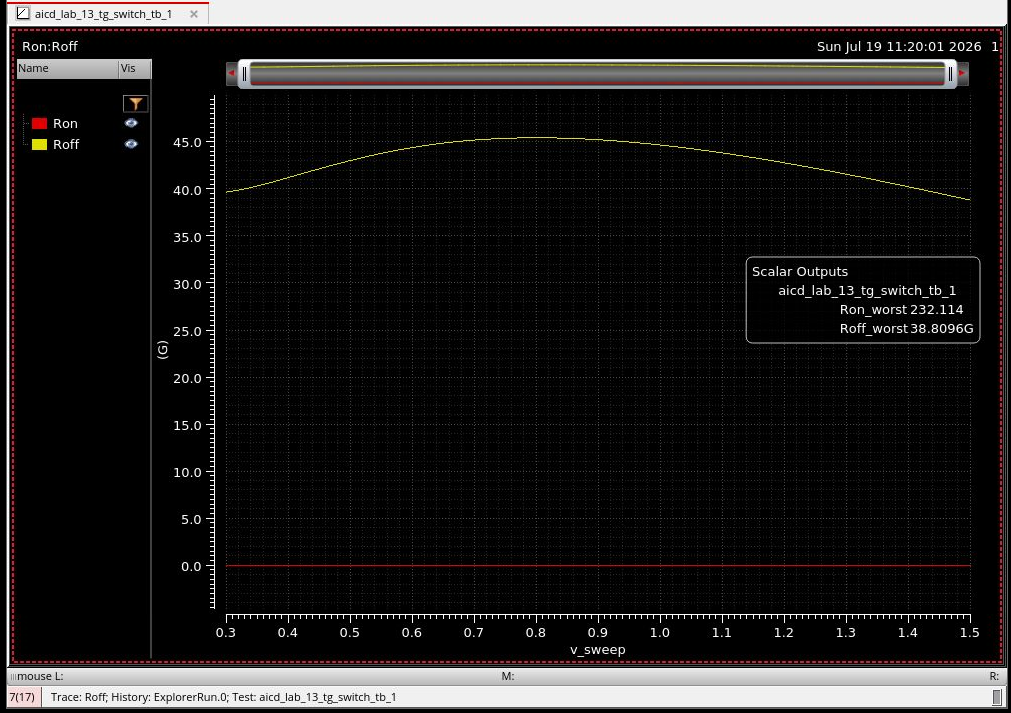
\includegraphics[width=\linewidth]{figures/pga/tg_resistance.png}
\end{minipage}
\caption{Nominal PGA gain versus digital code and transmission-gate resistance over the \SIrange{0.3}{1.5}{V} input sweep. Exact resistance limits are reported in the text.}
\label{fig:pga-gain-tg}
\end{figure}

\section{Active low-pass filter}

The second inverting stage uses equal input and feedback resistance. Each path contains four series RNHR elements of approximately \SI{401.65}{k\ohm}, giving approximately \SI{1.6066}{M\ohm} per path. The \SI{884.64}{fF} feedback capacitor is connected through an enable transmission gate.

Ignoring the enable-switch resistance and finite OPAMP response, the transfer function and pole are
\begin{align}
H(j\omega)
&=-\frac{R_2/R_1}{1+j\omega R_2 C}, \\
f_{\mathrm{p,ideal}}
&=\frac{1}{2\pi R_2 C}
\approx\SI{111.98}{kHz}.
\end{align}
The large resistance lets us reach the target time constant with the implemented \SI{884.64}{fF} capacitor. Reducing the total below the course guideline of approximately \SI{1}{M\ohm} would require a larger capacitor and a coordinated redesign of the filter, layout, and simulations. We therefore retained the \SI{1.6066}{M\ohm} value and treat it as an area and layout risk. The enable-switch resistance and finite OPAMP response shift the simulated -3 dB bandwidth to \SI{100.1}{kHz}, approximately \SI{10.6}{\percent} below the first-order estimate and within the allowed \SIrange{50}{150}{kHz} range.

% TODO(figure readability): Replace the LPF magnitude and phase panels with larger native exports if available. The curves are readable at the current scale, but the exact -3 dB value should be taken from the scalar result rather than the screenshot.
\begin{figure}[htbp]
\centering
\begin{minipage}[t]{0.48\textwidth}
\centering
\textbf{(a) Magnitude and -3 dB crossing}\par\smallskip
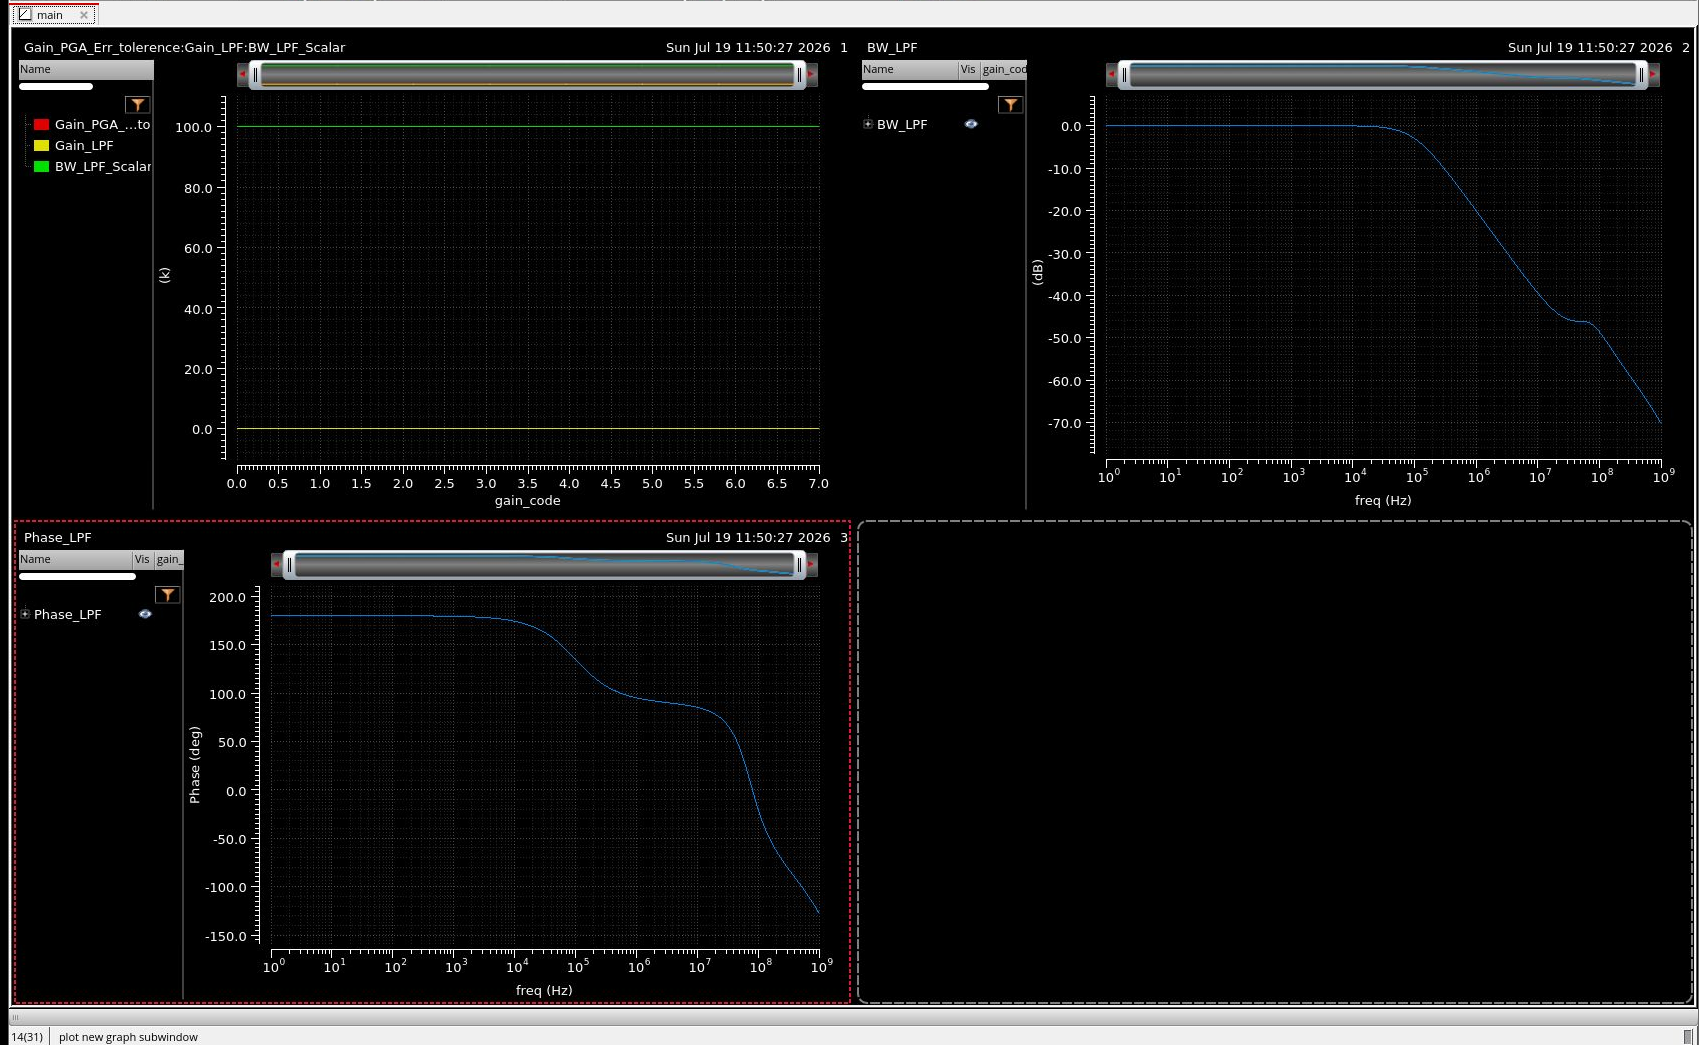
\includegraphics[width=\linewidth,trim=850 523 0 0,clip]{figures/pga/lpf_response.png}
\end{minipage}\hfill
\begin{minipage}[t]{0.48\textwidth}
\centering
\textbf{(b) Phase}\par\smallskip
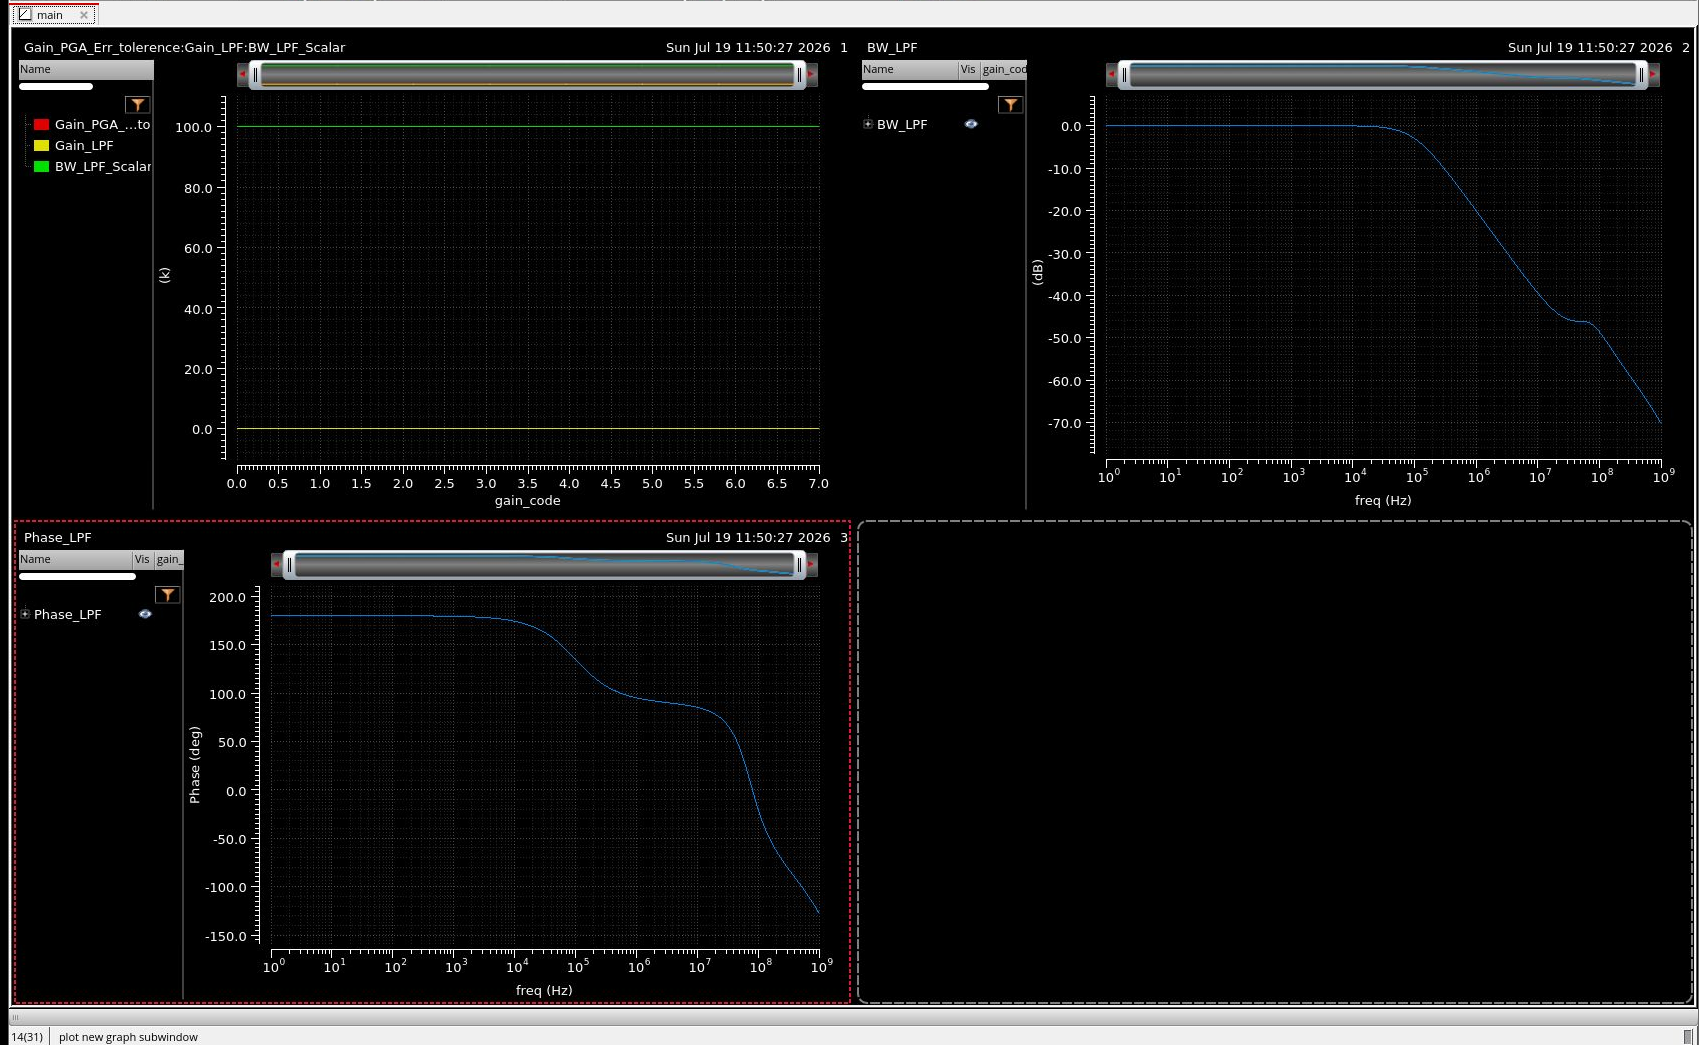
\includegraphics[width=\linewidth,trim=0 0 849 522,clip]{figures/pga/lpf_response.png}
\end{minipage}
\caption{Nominal LPF magnitude and phase response. The low-frequency phase near \SI{180}{\degree} is consistent with an inverting stage; the scalar -3 dB bandwidth is \SI{100.1}{kHz}.}
\label{fig:lpf-response}
\end{figure}

\section{Nominal, corner, and Monte Carlo results}

% LAYOUT HANDOFF: Add post-layout data to Tables 7(a) and 7(b) in the form
% PEX (schematic). Use the same eight codes, 64-corner grid, and 100 Monte
% Carlo points per code. Keep all schematic values unchanged. The LPF PEX
% comparison belongs in chapters/layout.tex and should not be repeated here.

The nominal sweep covers \texttt{gain\_code=0:1:7} from \SI{1}{Hz} to \SI{1}{GHz} with 80 logarithmic points per decade. PGA gain is evaluated at \SI{1}{kHz} relative to the target $3\,\texttt{gain\_code}$. All eight nominal gains satisfy the $\pm\SI{1.5}{dB}$ window. An independent rerun changes the reported errors by no more than \SI{0.0142}{dB} and does not change the pass status.

Across 64 PVT corners, every PGA code and both LPF scalar checks pass. The largest PGA excursion is \SI{1.221}{dB} at code 000, leaving \SI{0.279}{dB} to the upper limit. The LPF bandwidth spans \SIrange{72.88}{121.8}{kHz}.

\begin{table}[H]
\centering
\caption{Course Table~7(a), schematic values for codes 000--011.}
\label{tab:pga-table7-low}
\scriptsize
\renewcommand{\arraystretch}{0.92}
\begin{tabularx}{\textwidth}{@{}Yrrrr@{}}
\toprule
Parameter & 000 (dB) & 001 (dB) & 010 (dB) & 011 (dB) \\
\midrule
Target / corner tolerance & $0\pm1.5$ & $3\pm1.5$ & $6\pm1.5$ & $9\pm1.5$ \\
Typical & 0.1463 & 3.1058 & 6.0723 & 9.0475 \\
Corner minimum & 0.0500 & 3.0319 & 6.0165 & 9.0117 \\
Corner maximum & 1.2210 & 3.8869 & 6.6357 & 9.4463 \\
Passed / total corners & 64/64 & 64/64 & 64/64 & 64/64 \\
\midrule
MC minimum & 0.0793 & 3.0511 & 6.0249 & 8.9976 \\
MC maximum & 0.2248 & 3.1748 & 6.1417 & 9.1179 \\
MC mean & 0.1461 & 3.1059 & 6.0721 & 9.0474 \\
MC standard deviation & 0.02701 & 0.02387 & 0.02253 & 0.02347 \\
MC yield & 100/100 & 100/100 & 100/100 & 100/100 \\
\bottomrule
\end{tabularx}
\end{table}

\begin{table}[H]
\centering
\caption{Course Table~7(b), schematic values for codes 100--111.}
\label{tab:pga-table7-high}
\scriptsize
\renewcommand{\arraystretch}{0.92}
\begin{tabularx}{\textwidth}{@{}Yrrrr@{}}
\toprule
Parameter & 100 (dB) & 101 (dB) & 110 (dB) & 111 (dB) \\
\midrule
Target / corner tolerance & $12\pm1.5$ & $15\pm1.5$ & $18\pm1.5$ & $21\pm1.5$ \\
Typical & 12.0304 & 15.0165 & 18.0059 & 20.9967 \\
Corner minimum & 12.0049 & 14.9998 & 17.9823 & 20.9546 \\
Corner maximum & 12.3129 & 15.2094 & 18.1299 & 21.0980 \\
Passed / total corners & 64/64 & 64/64 & 64/64 & 64/64 \\
\midrule
MC minimum & 11.9758 & 14.9724 & 17.9524 & 20.9303 \\
MC maximum & 12.0878 & 15.0652 & 18.0525 & 21.0686 \\
MC mean & 12.0292 & 15.0152 & 18.0055 & 20.9966 \\
MC standard deviation & 0.02074 & 0.02022 & 0.02069 & 0.02288 \\
MC yield & 100/100 & 100/100 & 100/100 & 100/100 \\
\bottomrule
\end{tabularx}
\end{table}

The Monte Carlo analysis uses variation \texttt{All}, 100 points per code, standard random sampling, seed 12345, and first point 1. All PGA and LPF outputs pass 100/100 points. PGA standard deviation is \SIrange{0.02022}{0.02701}{dB}. LPF bandwidth is \SIrange{82.8}{119.5}{kHz}, with a \SI{100.0}{kHz} mean and \SI{6.796}{kHz} standard deviation.

The archive contains no full all-code PGA AC magnitude/phase export or measured \texttt{010} to \texttt{101} switching waveform. The static sweeps support the tabulated gains; dynamic switching remains unverified.

\chapter{Scope and Remaining Work}

This portfolio presents schematic design and verification. Physical implementation was assigned to the teammate. Their layout images and DRC/LVS screenshots are omitted from the shared files; the contribution statement preserves that task split without displaying their implementation.

No completed OPAMP, PGA, or LPF extracted-view performance is claimed. The schematic results in the earlier chapters are not post-layout results. Area is not reported because no measured dimensions are included.

The recorded physical-verification flow was incomplete. Clean DRC and LVS, extraction, and matched schematic-to-PEX simulations would be needed before reporting post-layout nominal, corner, or Monte Carlo performance.

The schematic limitations also remain: the OPAMP output swing does not cover the full target range, and the offset Monte Carlo yield is 972/1000. The archive has no measured PGA gain-switching transient, full all-code PGA phase plot, or per-code summary of safe input range, stability, and power. Static code sweeps verify the behavioral decoder with the PGA feedback network; they do not establish switching-hazard or gate-level behavior.

The detailed device operating-point export is excluded from the shared repository. The compact operating-point table in the OPAMP chapter is retained to explain the design decisions. This editorial scope does not establish permission to redistribute technology data; any broader release needs confirmation of the applicable course and PDK terms.

\chapter{Conclusion}

The two-stage Miller-compensated OPAMP achieves \SI{79.93}{dB} DC gain, a \SI{51.31}{MHz} gain-bandwidth product, and a \SI{61.97}{\degree} phase margin. Within the specified \SIrange{0.5}{1.3}{V} ICMR, the maximum follower error is \SI{0.8503}{mV}. All 12 expressions in the 64-corner export pass at every corner. In the 1000-point Monte Carlo analysis, the offset meets the \SI{5}{mV} limit in 972 cases; the other exported metrics pass 1000/1000.

All eight PGA settings from 0 to \SI{21}{dB} in \SI{3}{dB} steps remain within the \(\pm\SI{1.5}{dB}\) tolerance at nominal conditions, across all 64 corners, and for 100 Monte Carlo samples per code. The behavioral Verilog-A controller is included in these complete PGA sweeps, which verify its static decode path together with the MUX and feedback network. The active LPF has a nominal bandwidth of \SI{100.1}{kHz}, with a corner range of \SIrange{72.88}{121.8}{kHz} and a Monte Carlo range of \SIrange{82.8}{119.5}{kHz}.

The remaining circuit-level limitation is the OPAMP output swing of approximately \SIrange{0.430}{1.401}{V}, which does not cover the full specified \SIrange{0.3}{1.5}{V} range. It caused no failure in the available PGA corner or Monte Carlo runs, so we retained the design for the tested operating range. We also retained the \SI{1.6066}{M\ohm} LPF resistance paths, accepting the resulting area risk instead of redesigning the capacitor and rerunning the complete flow.

This portfolio presents schematic design and verification. Physical implementation was assigned to the teammate; their layout images and verification screenshots are omitted. No complete extracted-view or PEX performance is claimed.

\section*{Contribution / Task Distribution}

Qi Wu carried out OPAMP integration, transistor sizing and tuning, and testbench setup. He designed the PGA feedback network and active LPF, integrated the transmission gates and behavioral Controller, and performed the final schematic-level verification and result analysis. The teammate designed the current-source and bias section, performed the initial PGA corner and Monte Carlo runs, and implemented the available component layouts and physical checks. Qi Wu prepared the layout handoff, wrote the schematic sections, and integrated the final report. The detailed task split is documented in the repository contribution statement. Results without supporting files are left open and explained in the corresponding section.

\chapter{Declaration of AI-Assisted Work}

Table~\ref{tab:ai-use} summarizes the use of AI in preparing the report. We created the circuits and simulations, supplied the technical content, and remain responsible for the final wording and results.

\begin{table}[htbp]
\centering
\caption{AI-assistance disclosure for the complete project report.}
\label{tab:ai-use}
\small
\begin{tabularx}{\textwidth}{@{}Y Y Y Y Y@{}}
\toprule
Type of application & Affected parts & Student contribution & AI tool & Remark \\
\midrule
Language and structure editing & abstract, scope, captions, contribution statement, and conclusion & Supplied the technical content; reviews the final wording & OpenAI Codex & No measurement was generated by AI \\
Numerical consistency checking & simulation tables, limits, statistics, and units & Created the designs and simulations; checks the Cadence exports & OpenAI Codex & Exported values remain the reference \\
LaTeX and PDF formatting & tables, figures, compilation, and page layout & Selects the content; reviews the compiled report & OpenAI Codex & Portfolio edition uses a standard LaTeX report class \\
\bottomrule
\end{tabularx}
\end{table}

\appendix
\chapter{Supporting OPAMP Evidence}

\begin{figure}[H]
\centering
\begin{minipage}[t]{0.38\textwidth}
\centering
\textbf{(a) Hand calculation, upper half}\par
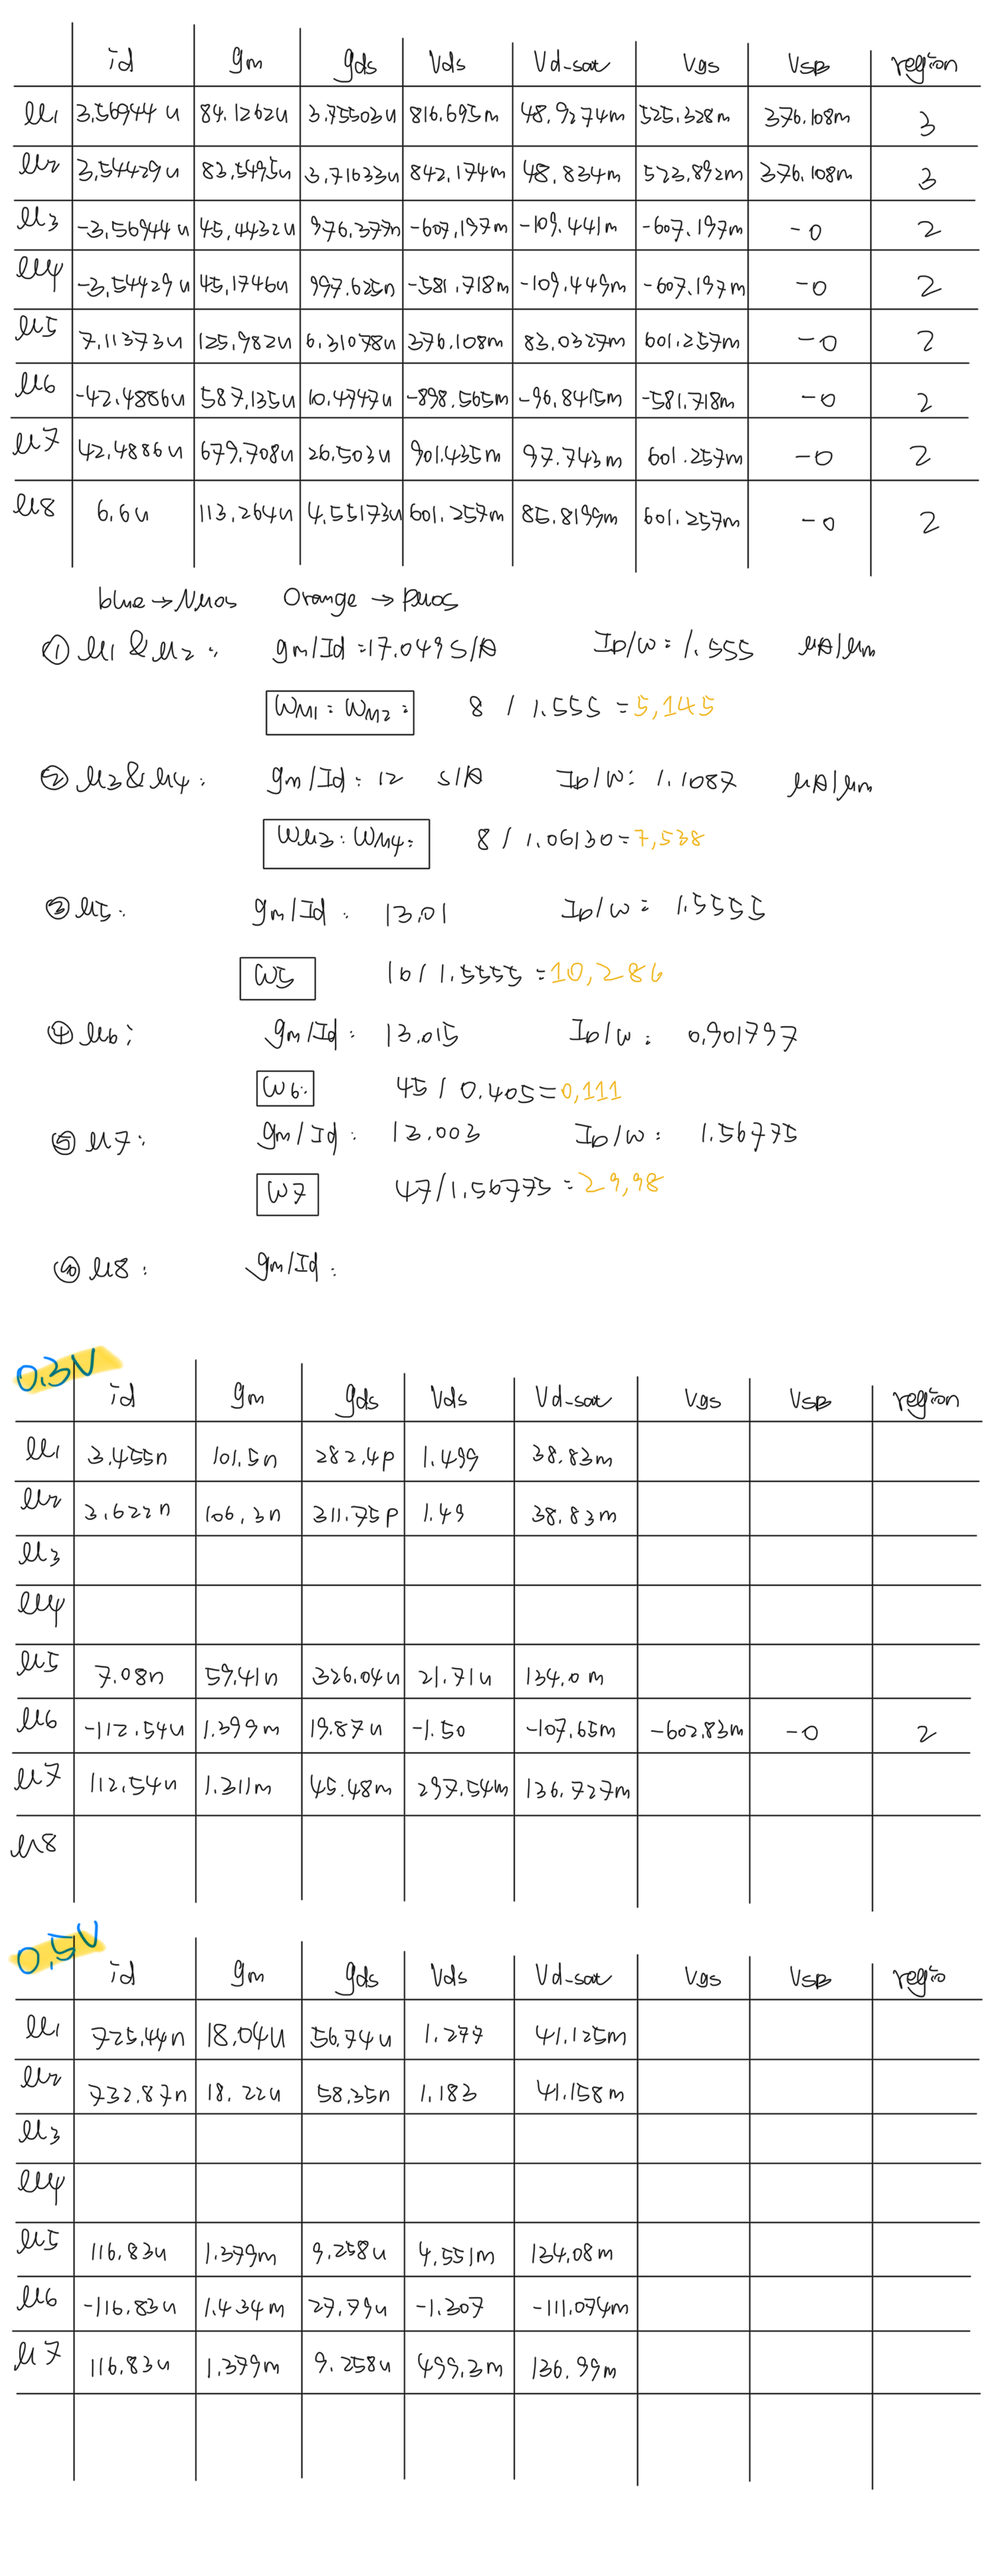
\includegraphics[width=\linewidth,trim=0 1538 0 0,clip]{figures/opamp/hand_calculation.png}
\end{minipage}\hfill
\begin{minipage}[t]{0.38\textwidth}
\centering
\textbf{(b) Hand calculation, lower half}\par
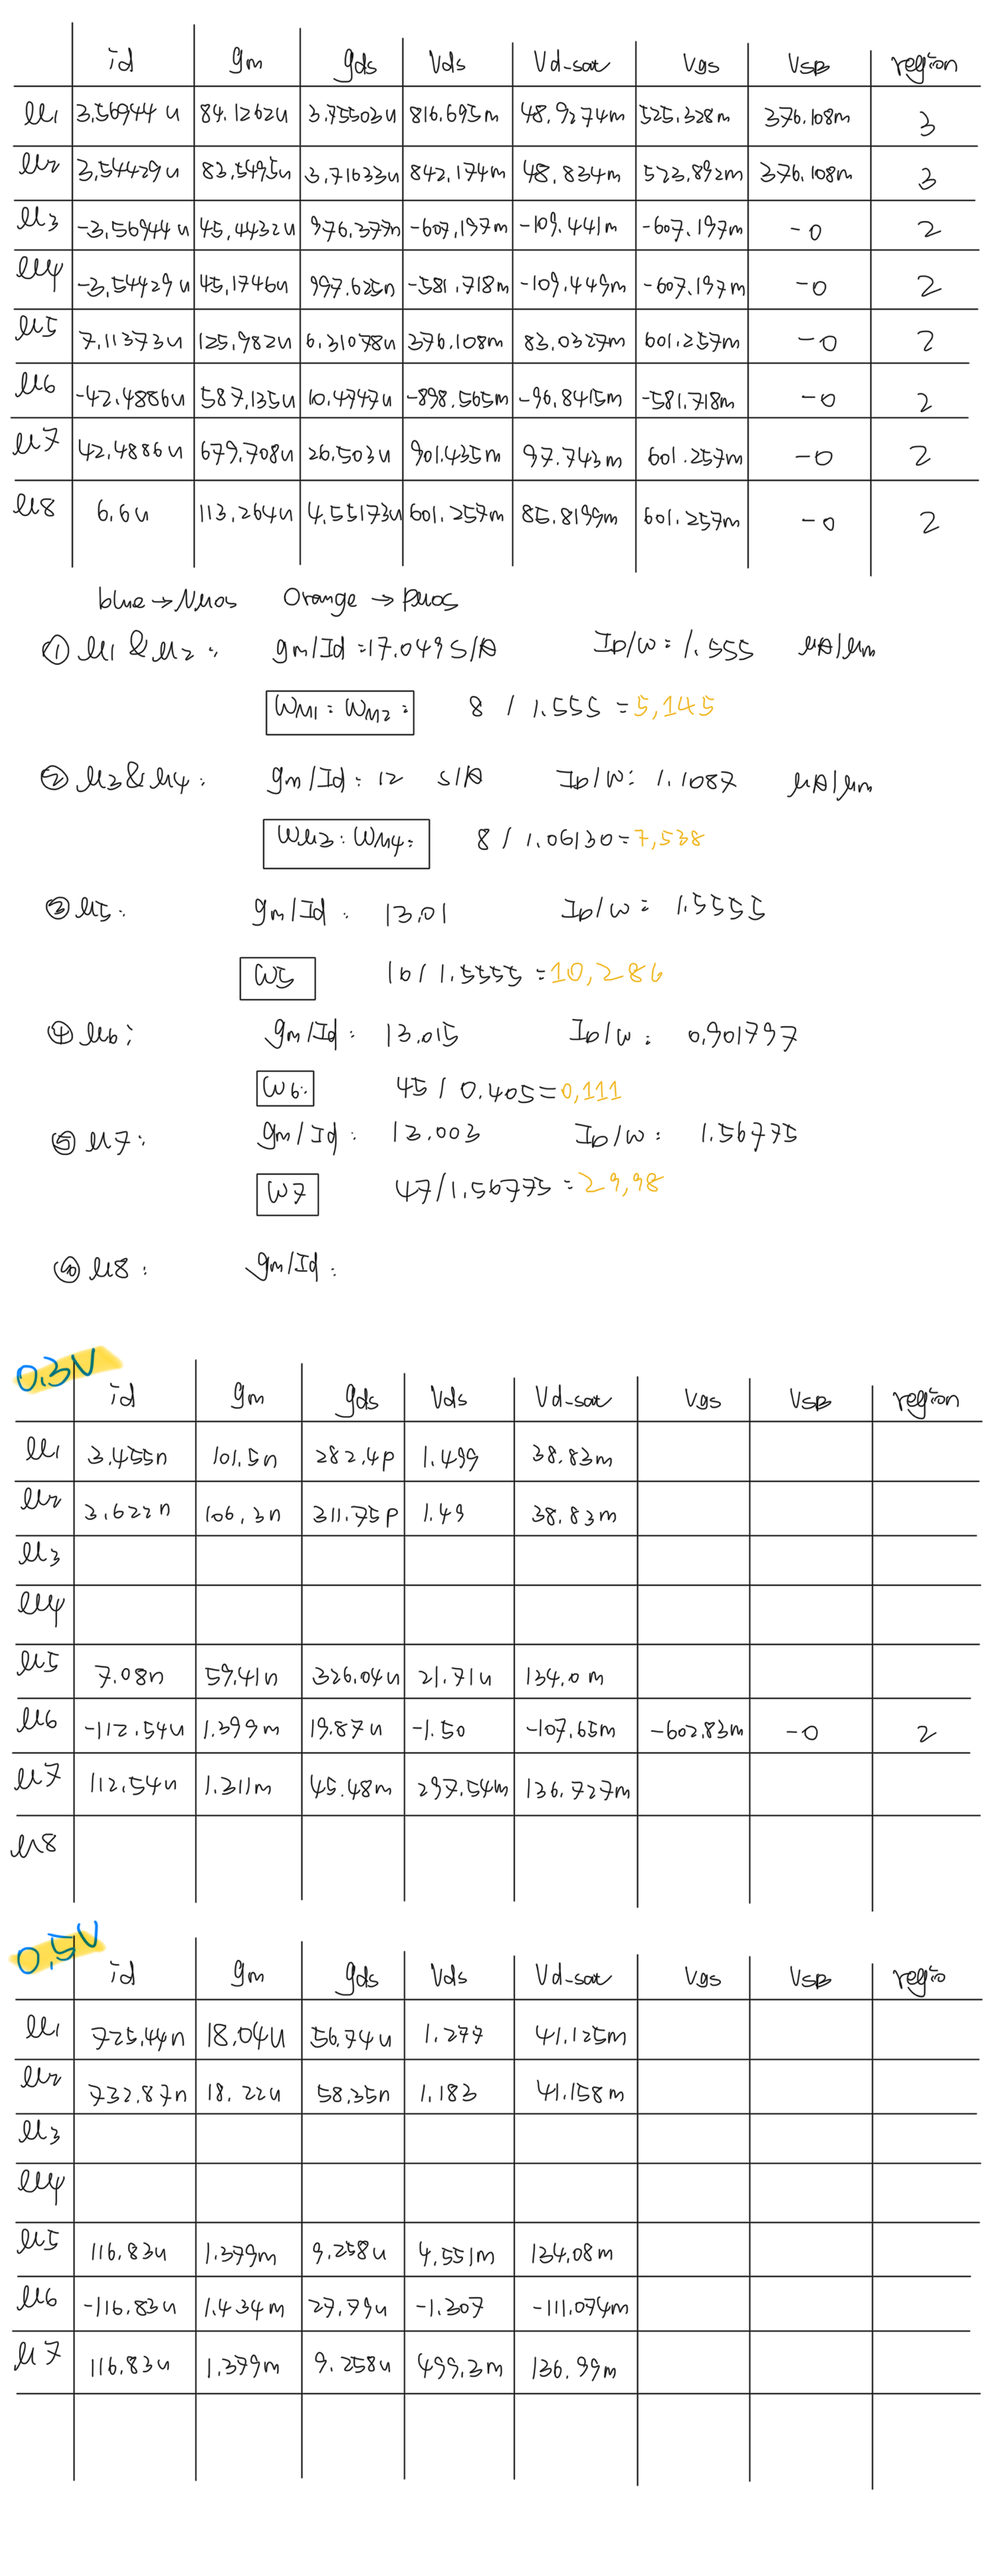
\includegraphics[width=\linewidth,trim=0 0 0 1538,clip]{figures/opamp/hand_calculation.png}
\end{minipage}

\begin{minipage}[t]{0.28\textwidth}
\centering
\textbf{(c) Corner setup}\par
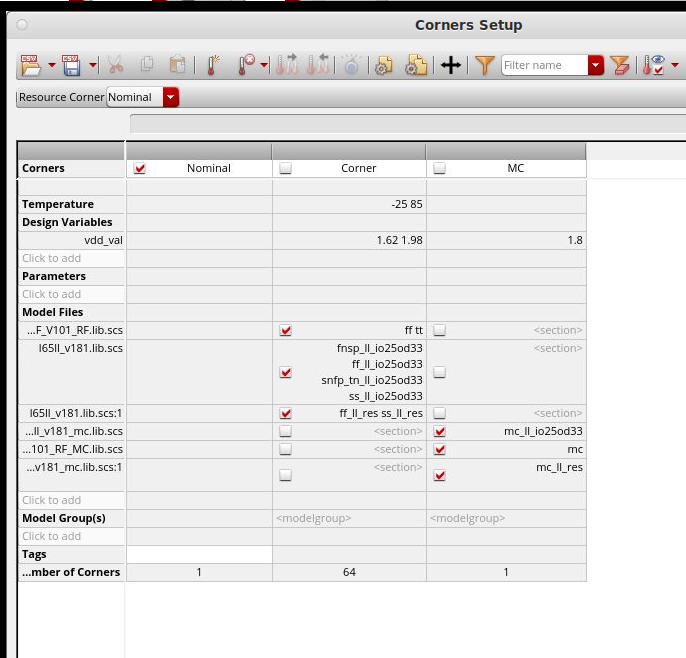
\includegraphics[width=\linewidth]{figures/opamp/corner_setup.png}
\end{minipage}\hfill
\begin{minipage}[t]{0.48\textwidth}
\centering
\textbf{(d) Offset Monte Carlo}\par
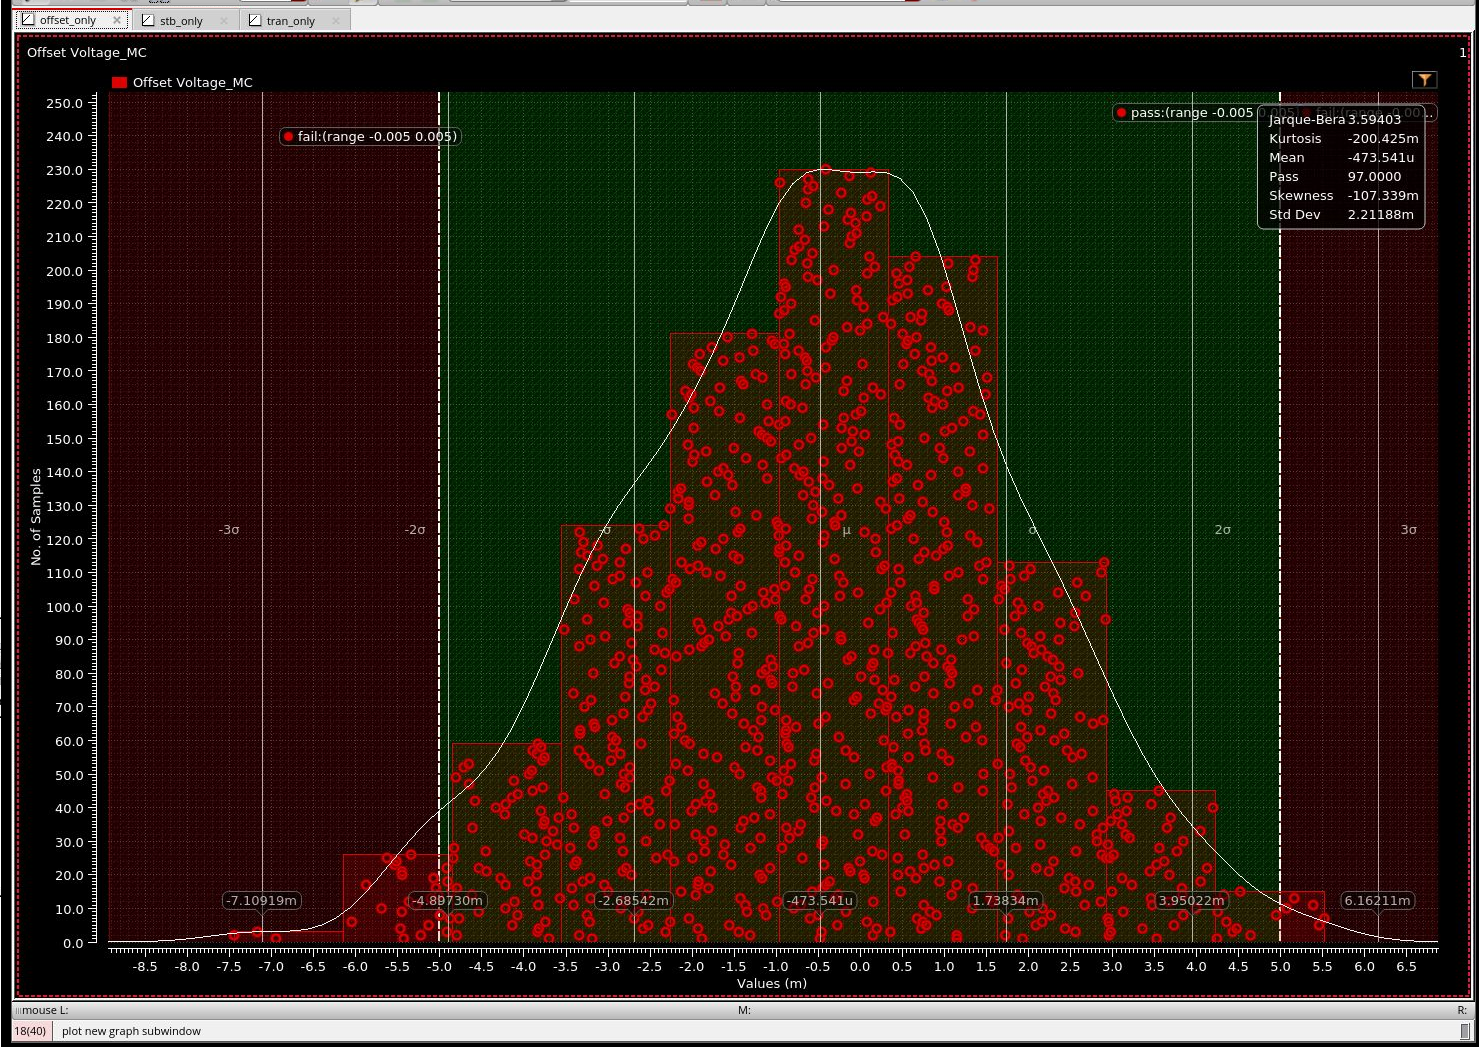
\includegraphics[width=\linewidth]{figures/opamp/mc_offset_histogram.png}
\end{minipage}
\caption{Supporting OPAMP evidence: hand calculations, the 64-corner setup, and the offset Monte Carlo distribution.}
\label{fig:opamp-supporting-evidence}
\end{figure}

\begingroup
\small
\listoffigures
\listoftables
\endgroup
\end{document}
